\section[{Моделирование динамических процессов в ледовом острове}]{Моделирование динамических процессов\\в ледовом острове}

\subsection{Постановка задачи}

Рассмотрим двумерную модель ледового острова шириной 300 м и высотой 10 м, покоящегося на дне моря глубиной 8 м.  Грунт под островом будем считать состоящим из придонного слоя глубиной 10 м и слоя осадочных пород глубиной 600 м. В некоторых случаях мы будем также рассматривать  газоносный слой, находящийся под слоем осадочных пород.  

В \autoref{tab:geo} приведены скорости поперечных и продольных волн $c_p$ в рассматриваемых средах, а также их плотность $\rho$.

Ставятся следующие задачи:

\begin{enumerate}
    \item Исследовать распространение акустических и упругих волн от бура, расположенного посередине длины острова на глубине 20 м, с учётом наличия газоносного слоя.
    
    \begin{figure}[htb]
        \centering
        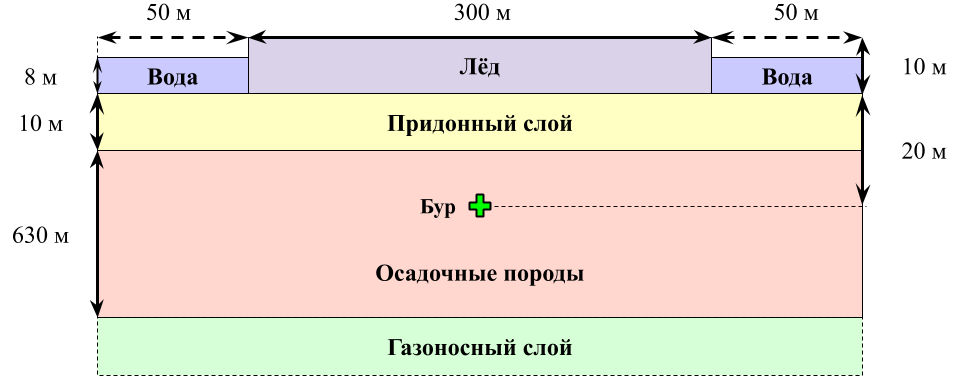
\includegraphics[width=0.8\textwidth]{images/gas_field/gas_field_scheme.png}
        \caption{Постановка задачи о бурении.}
        \label{fig:island}
    \end{figure}

    \item Найти распределение напряжений в ледовом острове при наличии здания на поверхности острова\footnote{Здесь линейные размеры слоёв совпадают с задачей о бурении, если не указано обратное.}. Оценить максимальную величину статической нагрузки, которая не приводит к разрушению льда. Найти области острова, наиболее подверженные разрушению.
    
    \begin{figure}[htb]
        \centering
        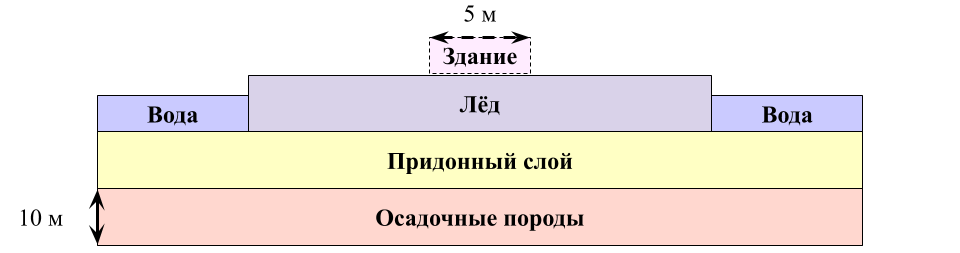
\includegraphics[width=0.8\textwidth]{images/stamp/stamp_scheme.png}
        \caption{Постановка задачи о статической нагрузке.}
        \label{fig:stamp_scheme}
    \end{figure}
\end{enumerate}

\renewcommand{\arraystretch}{1.2}
\begin{table}[htb]
\centering
    \begin{tabular}{|l|c|c|c|}
    \hline
    Среда & $c_p$, м/с & $c_s$, м/с & $\rho$, кг/м\textsuperscript{3} \\ \hline
    Лёд & 3940 & 2493 & 917 \\ \hline
    Вода & 1500  & --- & 1025 \\ \hline
    Придонный грунт & 1806 & 316 & 2000 \\ \hline
    Осадочные породы & 2250 & 1000 & 2000 \\ \hline
    \end{tabular}
\caption{Параметры рассматриваемых сред.}
\label{tab:geo}
\end{table}
\renewcommand{\arraystretch}{1.0}

\subsection{Математическая модель среды}

\subsubsection{Уравнения}

Рассматриваемые среды будем считать сплошными, однородными, изотропными и несжимаемыми. В описанной постановке присутствуют как жидкие среды (вода, окружающая остров), так и твёрдые среды (лёд и слои грунта).

Жидкие среды в двумерном случае в декартовой эйлеровой системе координат описываются системой уравнений акустики \cite{favorskaya_thesis}

\begin{equation}
    \begin{dcases}
        \rho \frac{\partial \vec{v}(x,y,t)}{\partial t} = -\nabla p (x,y,t) ,\\
        \frac{\partial p(x,y,t)}{\partial t} = -\rho c^2 \Div \vec{v}(x,y,t) ,
    \end{dcases}
    \label{eq:acoustic_wave_eq}
\end{equation}

\noindent где $\rho$ --- плотность среды, $\vec{v}(x,y,t)$ --- вектор скорости (производная вектора смещения частицы среды $\vec{u}(x,y,t)$ по времени), $p(x,y,t)$ --- давление, $c$ --- скорость звука в жидкости.

Твёрдые среды в двумерном случае в декартовой эйлеровой системе координат описываются уже системой уравнений линейно-упругой среды \cite{favorskaya_thesis}

\begin{equation}
    \begin{dcases}
        \rho \frac{\partial \vec{v}(x,y,t)}{\partial t} = \Div^T \pmb{\sigma} (x,y,t) , \\
        \!\begin{aligned}
            \frac{\partial \pmb{\sigma}(x,y,t)}{\partial t} & = \rho \left(c_p^2 - 2c_s^2\right) \Div \vec{v}(x,y,t) \ \pmb{I} +\\
            & +\rho c_s^2 \left(\nabla \otimes \vec{v}(x,y,t) + \left[ \nabla \otimes \vec{v}(x,y,t)\right]^T \right),
        \end{aligned} 
    \end{dcases}
    \label{eq:elastic_wave_eq}
\end{equation}

\noindent где $\pmb{\sigma}(x,y,t)$ --- симметричный тензор напряжений Коши второго ранга, $c_p$ и $c_s$ --- скорости продольной и поперечной волн соответственно, $\pmb{I}$ --- единичный тензор второго ранга, операция $\otimes$ --- тензорное произведение векторов.

Далее мы будем для краткости опускать значок у вектора скорости, т.е. будем писать $v$, подразумевая при этом вектор $\vec{v}$. Также мы будем опускать параметры $(x,y,t)$ у зависящих от них величин.

\subsubsection{Контактные условия}

Контактные условия, изображённые на \autoref{fig:contacts}, одинаковы для задачи о бурении и задачи о статической нагрузке.

\begin{figure}[htb]
    \centering
    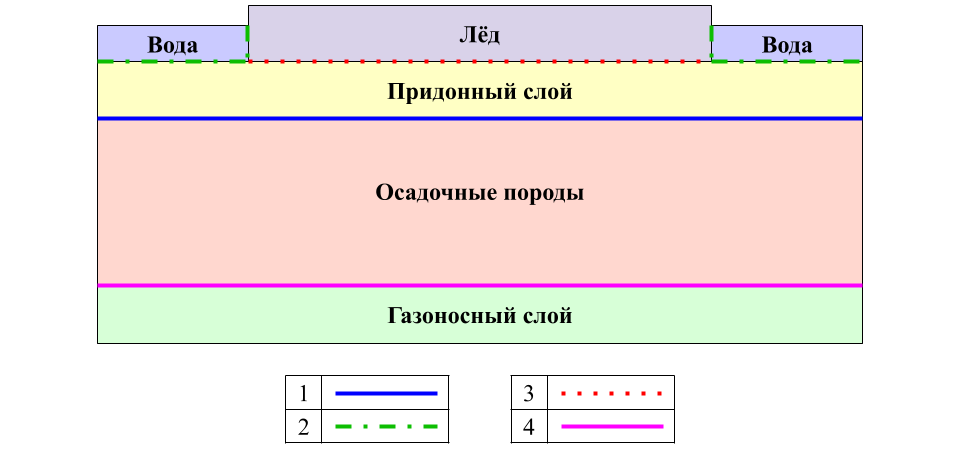
\includegraphics[width=0.8\textwidth]
    {images/gas_field/contacts.png}
    \caption{Схема контактных условий: 1 --- контактное условие полного слипания, 2 --- контактное условие между упругой и акустической средами, 3 --- контактное условие скольжения, 4 --- контактное условие отражения.}
    \label{fig:contacts}
\end{figure}

Здесь и далее мы будем обозначать контактирующие среды (или расчётные сетки) индексами $L$ и $R$ --- левая и правая среды соответственно. Вектор внешней нормали к левой под-области обозначим как $n$.

\begin{enumerate}
    \item Контактное условие полного слипания ставится между слоями твёрдых сред. Физически оно означает возможность беспрепятственного распространения упругих волн. Для этого требуется равенство скоростей и векторов нормального напряжения на границе раздела. Математически условие полного слипания записывается следующим образом:
    
    \begin{equation*}
    \begin{dcases}
        v_L = v_R ,\\
        \pmb{\sigma}_L \cdot n = \pmb{\sigma}_R \cdot n .
    \end{dcases}
    \end{equation*}
    
    \item Контактное условие между упругой и акустической средой используется для реализации перехода волн из твёрдых сред в жидкость и обратно. Оно отличается от условий полного слипания, т.к. в данном случае контактирующие среды описываются разными уравнениями (см. \eqref{eq:acoustic_wave_eq} и  \eqref{eq:elastic_wave_eq}).
    
    Если считать, что акустическая среда отвечает индексу $L$, а упругая --- $R$, то данное условие запишется как
    \begin{equation*}
    \begin{dcases}
        v_L \cdot n = v_R \cdot n , \\
        \pmb{\sigma} \cdot n + p n = 0 .
    \end{dcases}
    \end{equation*}
    
    Физически это условие означает не-протекание жидкости и твёрдой среды друг в друга.
    
    \item Контактное условие свободного скольжения ставится между ледовым островом и грунтом. В отличие от случая контакта двух слоёв грунта, когда применяется условие полного слипания, лёд и придонный слой могут двигаться друг относительно друга. Это явление известно на практике, так, например, наблюдается <<соскальзывание>> ледников с поверхностей гор. Таким образом требуется использование специального контактного условия:
    
    \begin{equation*}
    \begin{dcases}
        v_L \cdot n = v_R \cdot n , \\
        n \cdot \pmb{\sigma}_L \cdot n = n \cdot \pmb{\sigma}_R \cdot n, \\
        n \cdot \pmb{\sigma}_{L/R} \cdot n = \pmb{\sigma}_{L/R} \cdot n .
    \end{dcases}
    \end{equation*}
    
    \item Контактное условие полного отражения (свободной границы) ставится на границе раздела осадочных пород и газоносного слоя. Применение такого условия на верхней границе газоносного слоя не является вполне физически верным, однако для нашей задачи его применение вполне оправдано. Условие полного отражения имеет следующий вид:

    \begin{equation*}
        \pmb{\sigma} \cdot n = 0 .
    \end{equation*}
    
    Заметим, что для газоносного слоя не нужно вводить расчётную сетку --- в модели он представляется исключительно отражающим контактным условием.
\end{enumerate}

\subsubsection{Граничные условия}

Граничные условия для задачи о бурении изображены на \autoref{fig:borders}, для задачи о статической нагрузке --- на \autoref{fig:stamp_borders}.

\begin{figure}[htb]
    \centering
    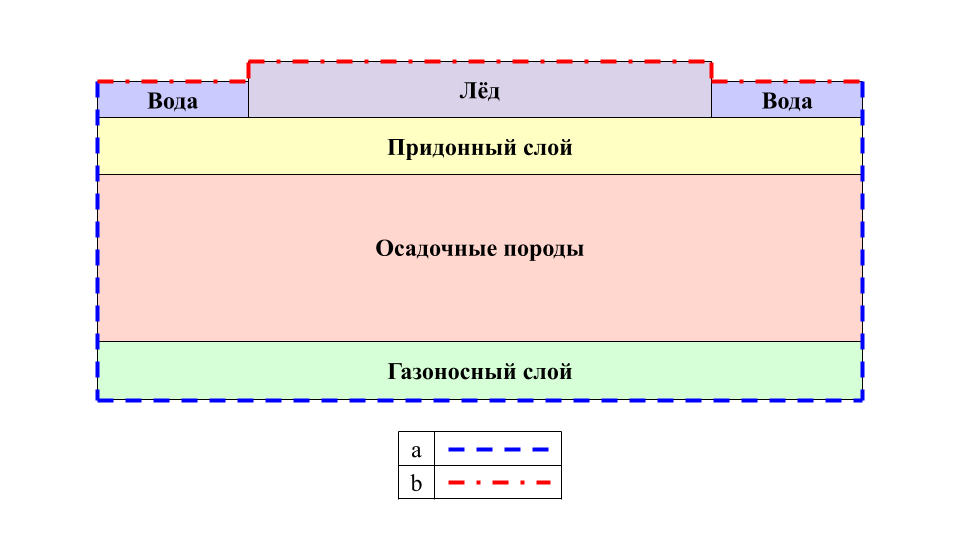
\includegraphics[width=0.8\textwidth]
    {images/gas_field/border_conds.png}
    \caption{Схема граничных условий для задачи о бурении: a --- граничное условие поглощения, b --- граничное условие нулевого давления.}
    \label{fig:borders}
\end{figure}

\begin{figure}[htb]
    \centering
    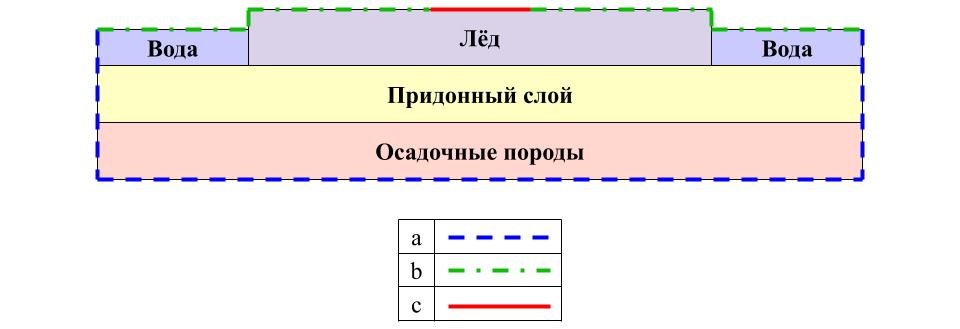
\includegraphics[width=0.8\textwidth]
    {images/stamp/stamp_border.png}
    \caption{Схема граничных условий для задаче о статической нагрузке: a --- граничное условие поглощения, b --- граничное условие нулевого давления, с --- граничное условие постоянного  давления.}
    \label{fig:stamp_borders}
\end{figure}

\begin{enumerate}[a.]
    \item Поглощающие (не-отражающие) граничные условия используются при рассмотрении ограниченной подобласти бесконечной физической области. В данном случае водяной, придонный, газоносный слои и слой осадочных пород продолжаются за границы расчётной области влево и вправо. Поэтому на их краях необходимо использовать поглощающие граничные условия.  Для упругих сред это условие запишется в виде:
    
    \begin{equation*}
    \begin{dcases}
        v_{l-2}^n = 
        v_{l-1}^n = 
        v_{l}^n , \\
        \pmb{\sigma}_{l-2}^n = 
        \pmb{\sigma}_{l-1}^n = 
        \pmb{\sigma}_{l}^n ,
    \end{dcases}
    \end{equation*}
    
    а для акустических сред в виде
    
    \begin{equation*}
    \begin{dcases}
        v_{l-2}^n = 
        v_{l-1}^n = 
        v_{l}^n ,\\
        p_{l-2}^n = 
        p_{l-1}^n = 
        p_{l}^n .
    \end{dcases}
    \end{equation*}
    
    Здесь верхний индекс $n$ обозначает момент времени $t_n$, а нижний --- номер сеточного узла, при этом узел $l$ является граничным, а узлы $l-1$ и $l-2$ --- его соседями по одной из осей. Такая форма записи будет верна и для левой, и для правой границы при соответствующем выборе значений координатных индексов.
    
    \item Граничное условие нулевого давления применяется на границе сред с воздухом. В нашей задаче мы не учитываем влияние атмосферного давления на исследуемые процессы, считая его пренебрежимо малым. Следовательно, мы принимаем $p=0$ на границах вода-воздух и лёд-воздух.
    
    \item Граничное условие постоянного давления ставится в месте контакта здания и ледового острова и записывается следующим образом:
    
    \begin{equation*}
    \begin{dcases}
        p = \sigma_{yy} = P_0, \\
        \sigma_{xx} = \sigma_{xy} = 0 .
    \end{dcases}
    \end{equation*}
    
    Здесь $P_0$ --- константа, равная давлению здания на поверхность льда.
\end{enumerate}

\subsubsection{Модель бура}

Современные буры имеют довольно сложное устройство, зачастую сочетая ударные и вращательные механизмы. В данной работе нас в первую очередь интересует волновая картина, возникающая при бурении в конкретной геологической модели (\autoref{fig:island}). Поэтому, для простоты, мы будем представлять воздействие бура в качестве точечного источника с импульсом Рикера частотой 30 Гц и амплитудным коэффициентом 10\textsuperscript{12} \cite{favorskaya_thesis}.

Точечный источник входит в левую часть системы уравнений \eqref{eq:gcm_system}, как слагаемое $\frac{R(t)}{\rho}$, и задаётся формулой

\begin{equation}
    R(t) =  \delta\left(r - r_0\right) R(t) \varphi ,
    %p(x,y) = \dfrac{1}{\pi \sigma^4} \left(1-\dfrac{1}{2}\left(\dfrac{x^2+y^2}{\sigma^2}\right)\right) \exp\left({-\frac{x^2+y^2}{2\sigma^2}}\right)
    \label{eq:ricker}
\end{equation}

\noindent где $r_0$ --- радиус-вектор положения точечного источника
\begin{equation*}
    r = \begin{pmatrix} x \\ y \end{pmatrix},
\end{equation*}

\noindent а $R(t)$ --- импульс Рикера частотой $f$ и коэффициентом сжатия $A$:

\begin{equation*}
    R(t) = A \left(1-2\pi^2 f^2 t^2\right) \exp \left(-\pi^2 f^2 t^2\right).
\end{equation*}

\begin{figure}[!htb]
\centering
    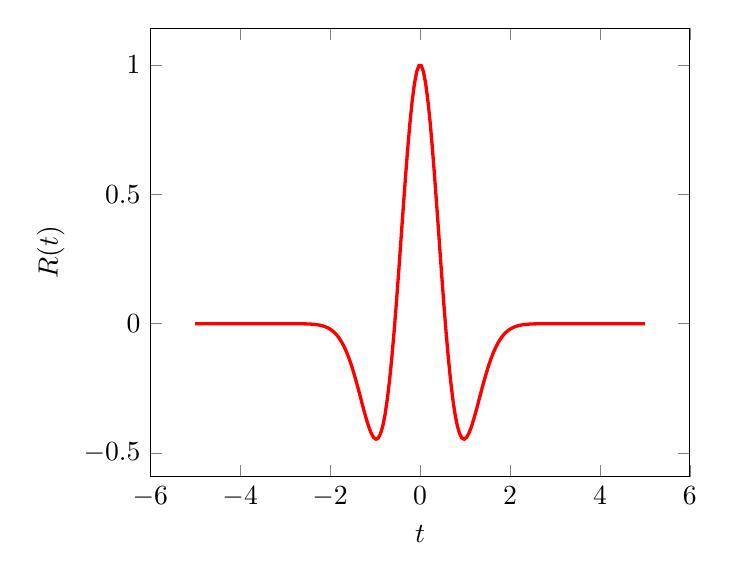
\begin{tikzpicture}
        \begin{axis}[
            xlabel = $t$,
            ylabel = {$R(t)$},
        ]
        \addplot[
            color      = red,
            line width = 1.2,
            samples    = 200
        ]
        {(1-2*(3.14^2)*(0.4^2)*(x^2))*exp(-(3.14^2)*(0.4^2)*(x^2))};
    \end{axis}
    \end{tikzpicture}
\caption{Импульс Рикера частотой 0.4 Гц и амлпитудным коэффициентом 1.}
\label{fig:ricker_plot}
\end{figure}
%\begin{figure}[htb]
%    \centering
%    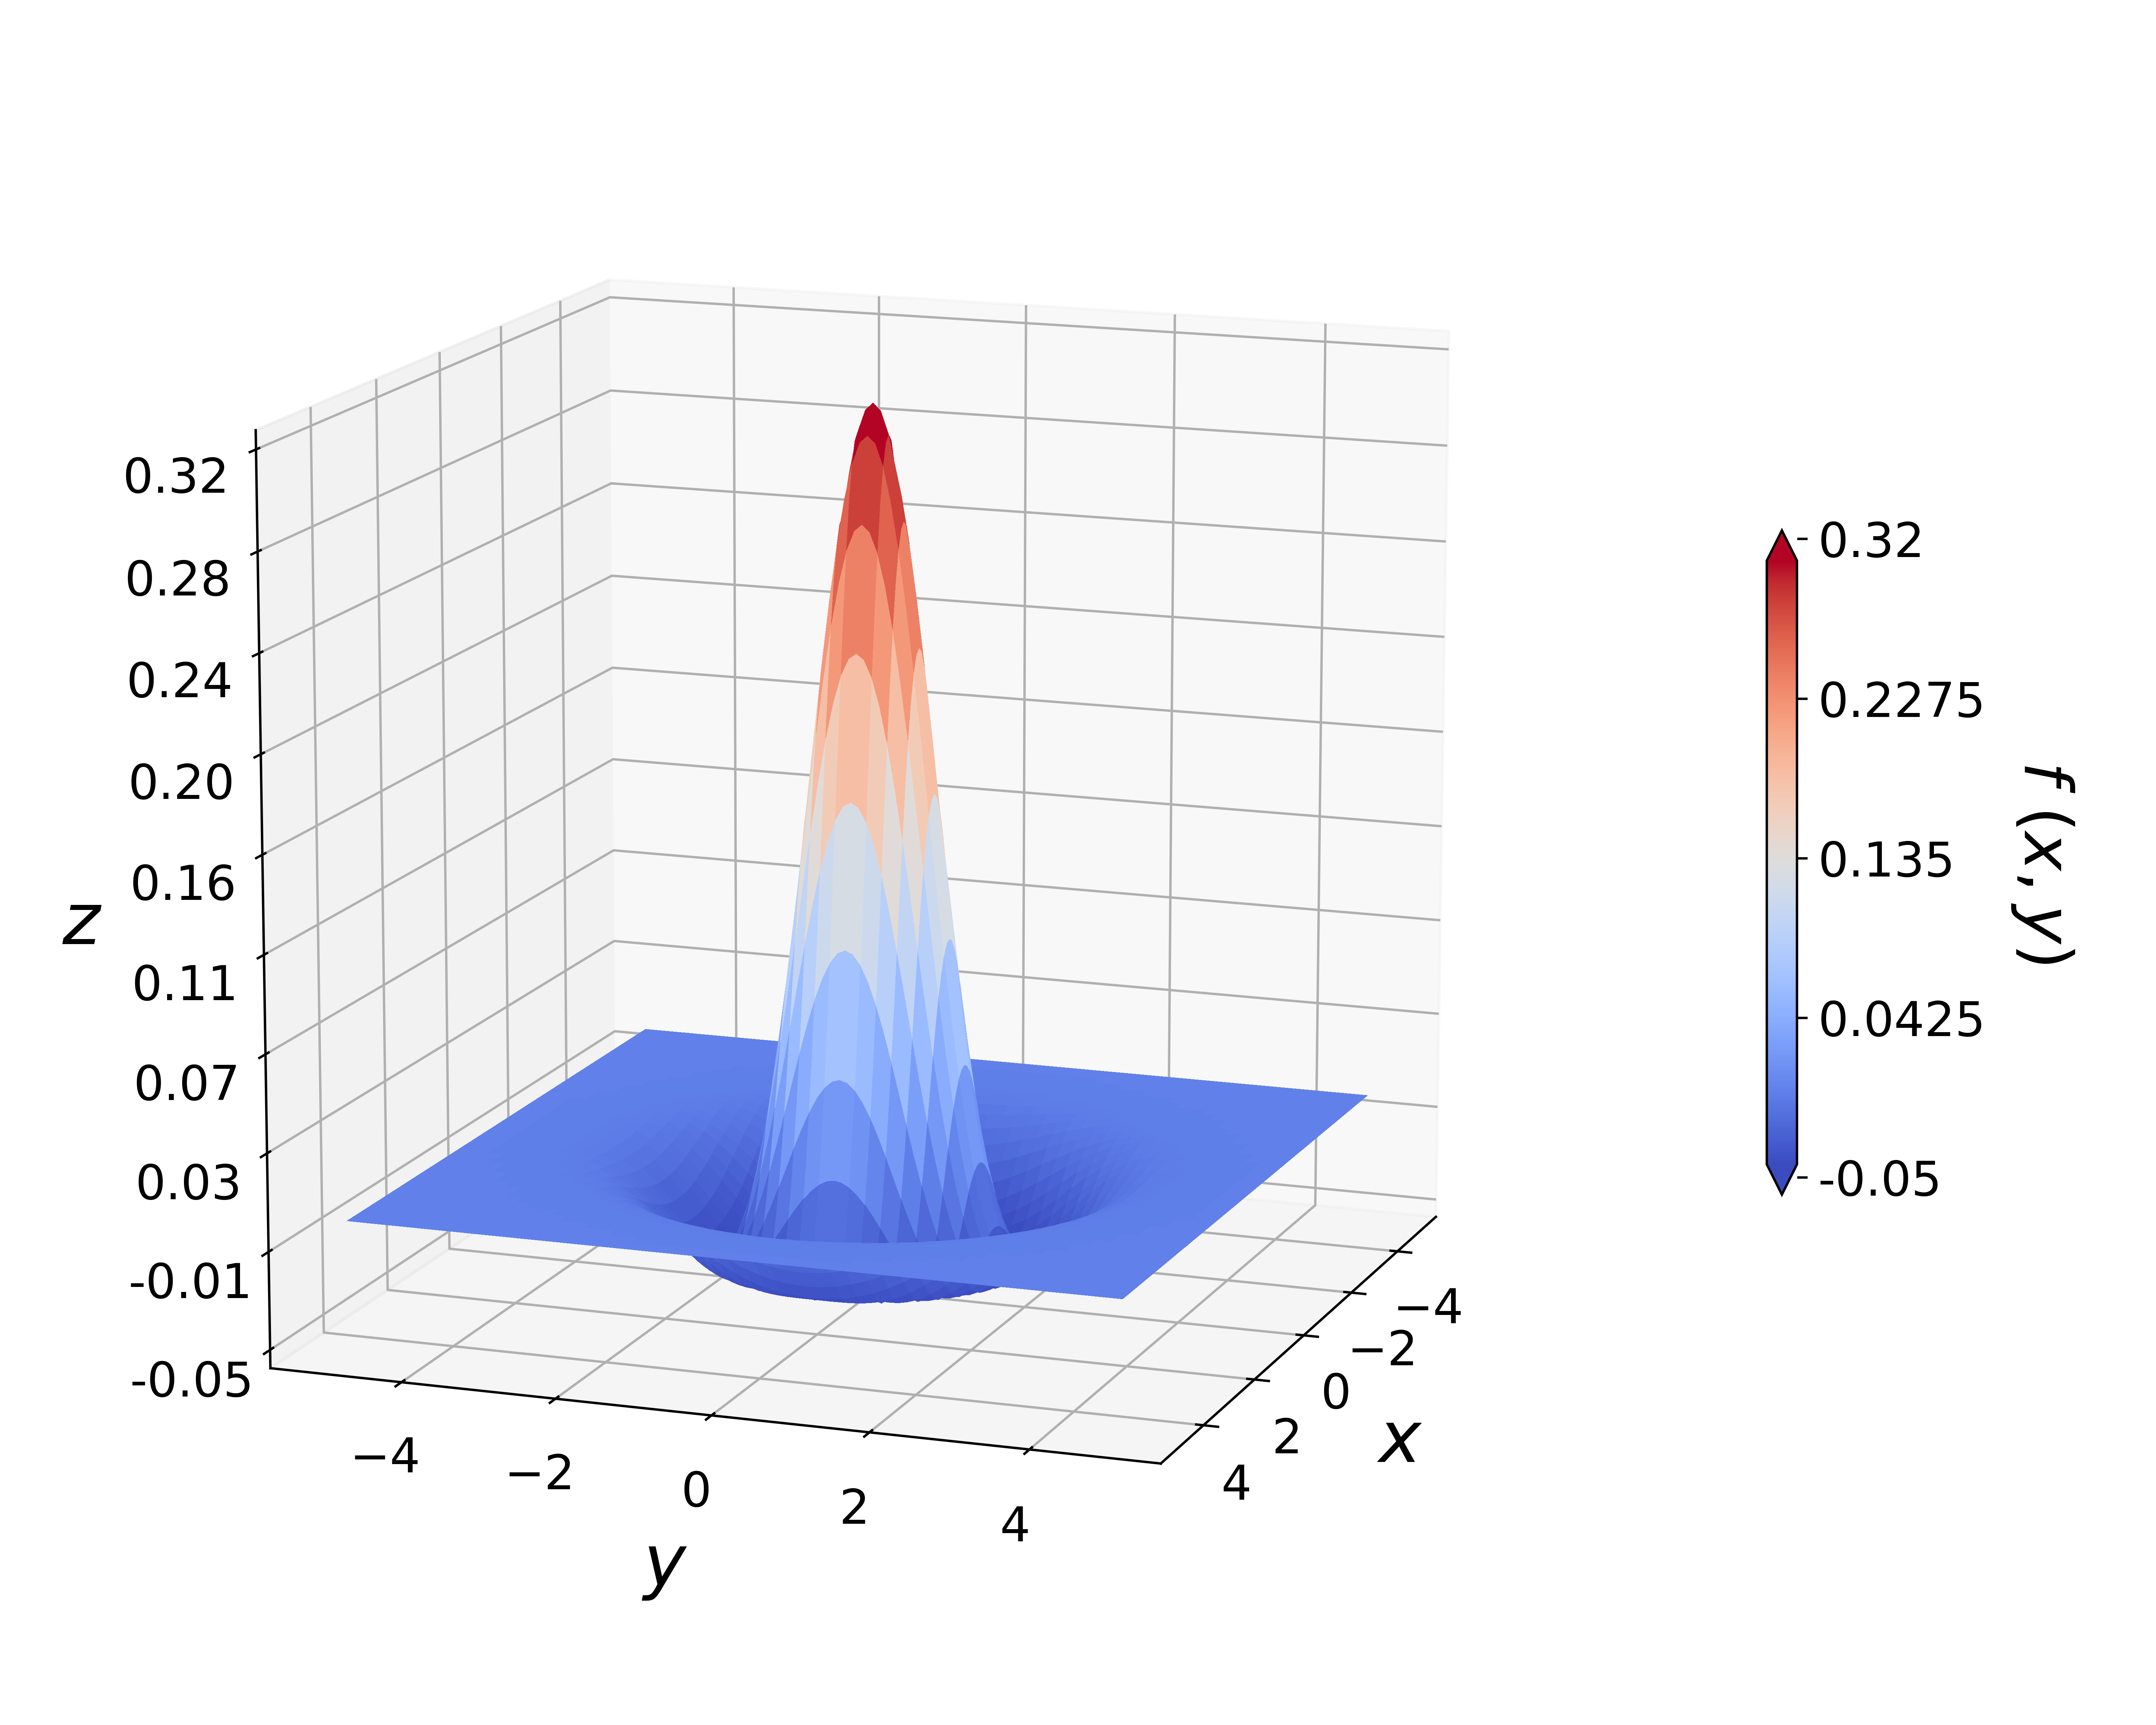
\includegraphics[trim={0px 45px 0px 80px},clip,width=0.7\textwidth]{images/gas_field/ricker_wavelet.png}
%    \caption{График импульса Рикера \eqref{eq:ricker} при $\sigma=1$.}
%    \label{fig:ricker_plot}
%\end{figure}

\subsubsection{Модель разрушений}

Для оценки прочности ледового острова будем использовать дискретную модель разрушений с критерием по главному напряжению \cite{grigoriev}. На каждом шаге для всех узлов сетки ледового острова будем вычислять напряжение фон Мизеса

\begin{equation*}
    \sigma_\nu = \sqrt{\dfrac{\left(\sigma_{xx} - p\right)^2 + \left(\sigma_{yy} - p\right)^2 + 2\sigma_{xy}^2}{2}} ,
\end{equation*}

\noindent где давление 
\begin{equation*}
    p=\frac{\sigma_{xx}+\sigma_{xy}+\sigma_{yy}}{3} .
\end{equation*}

\noindent Лёд разрушается, если выполнен критерий сдвигового разрушения

\begin{equation*}
    \sigma_\nu > y_s ,
\end{equation*}

\noindent где $y_s$ --- предел сдвигового напряжения, равный 1 МПа для льда.

\subsection{Численный метод}

\subsubsection{Сеточно-характеристический метод}
\label{sec:elastic_gcm}

Для решения систем уравнений в частных производных \eqref{eq:acoustic_wave_eq} и \eqref{eq:elastic_wave_eq}  воспользуемся сеточ\-но-характеристическим методом на регулярных прямоугольных сетках. Получим его для системы \eqref{eq:elastic_wave_eq}, описывающей упругие среды. Для системы \eqref{eq:acoustic_wave_eq}, описывающей акустические среды, он получается абсолютно аналогично если учесть, что для акустических сред $\sigma_{xx} = \sigma_{yy} = p$ и $\sigma_{xy}=0$.

Будем работать в декартовой прямоугольной системе координат. Введём обозначение

\begin{equation*}
    \varphi = \begin{pmatrix} v_x \\ v_y \\ \sigma_{xx} \\ \sigma_{xy} \\ \sigma_{yy} \end{pmatrix}
\end{equation*}

\noindent Здесь нижние индексы обозначают соответствующие компоненты вектора скорости $v$ и тензора напряжений $\pmb{\sigma}$.

Запишем гиперболическую полную систему линейных дифференциальных уравнений в частных производных \eqref{eq:elastic_wave_eq} в канонической матричной форме:

\begin{equation}
    \dfrac{\partial \varphi}{\partial t} + 
    \pmb{A} \dfrac{\partial \varphi}{\partial x} + 
    \pmb{B} \dfrac{\partial \varphi}{\partial y} = 0
    \label{eq:gcm_system}
\end{equation}.

\noindent Здесь

\begin{equation*}
    \pmb{A} = \begin{pmatrix}
        0 & 0 & -\frac{1}{\rho} & 0 & 0 \\
        0 & 0 & 0 & -\frac{1}{\rho} & 0 \\
        -(\lambda+2\mu) & 0 & 0 & 0 & 0 \\
        0 & -\mu & 0 & 0 & 0 \\
        -\lambda & 0 & 0 & 0 & 0
    \end{pmatrix},
\end{equation*}

\begin{equation*}
    \pmb{B} = \begin{pmatrix}
        0 & 0 & 0 & 0 & 0 \\
        0 & 0 & -\frac{1}{\rho} & 0 & 0 \\
        0 & -\lambda & 0 & 0 & 0 \\
        -\mu & 0 & 0 & 0 & 0 \\
        0 & -(\lambda+2\mu) & 0 & 0 & 0
    \end{pmatrix},
\end{equation*}

\noindent где $\lambda$ и $\mu$ --- параметры Ламе, которые выражаются через заданные для конкретных сред скорости продольных и поперечных волн следующим образом:

\begin{equation*}
    \begin{dcases}
        c_p = \sqrt{\dfrac{\lambda + 2\mu}{\rho}} \\
        c_s = \sqrt{\dfrac{\mu}{\rho}}
    \end{dcases}
    \quad \Rightarrow \quad
    \begin{dcases}
        \lambda = \left(c_p^2 - 2 c_s^2\right) \rho \\
        \mu = c_s^2 \rho 
    \end{dcases}
    .
\end{equation*}

\noindent Используя метод расщепления для системы, записанной в каноническом виде, получим систему

\begin{equation}
    \begin{dcases}
        \dfrac{\partial \varphi_x}{\partial t} + \pmb{A} \dfrac{\partial \varphi_x}{\partial x} = 0 , \\
        \dfrac{\partial \varphi_y}{\partial t} + \pmb{B} \dfrac{\partial \varphi_y}{\partial y} = 0 .
    \end{dcases}
    \label{eq:rashepl_elastic}
\end{equation}

\noindent Заметим, что матрицы $\pmb{A}$ и $\pmb{B}$ можно диагонализовать:
%https://www.wolframalpha.com/input/?i=%7B%7B0%2C0%2C-1%2Fp%2C0%2C0%7D%2C%7B0%2C0%2C0%2C-1%2Fp%2C0%7D%2C%7B-%28l%2B2m%29%2C0%2C0%2C0%2C0%7D%2C%7B0%2C-m%2C0%2C0%2C0%7D%2C%7B-l%2C0%2C0%2C0%2C0%7D%7D
%https://www.wolframalpha.com/input/?i=%7B%7B0%2C0%2C0%2C-1%2Fp%2C0%7D%2C%7B0%2C0%2C0%2C0%2C-1%2Fp%7D%2C%7B0%2C-l%2C0%2C0%2C0%7D%2C%7B-m%2C0%2C0%2C0%2C0%7D%2C%7B0%2C-%28l%2B2m%29%2C0%2C0%2C0%7D%7D

\begin{gather*}
    \pmb{A} = \pmb{S}^{-1}_1 \pmb{\Lambda}_1 \pmb{S}_1 , \\
    \pmb{B} = \pmb{S}^{-1}_2 \pmb{\Lambda}_2 \pmb{S}_2 ,
\end{gather*}

\noindent где

\begin{gather*}
    \pmb{S}_1 = 
    \begin{pmatrix}
        0 & 0 & 0 & 0 & 1 \\
        0 & \frac{\sqrt{\mu\rho}}{2} & 0 & \frac{1}{2} & 0 \\
        0 & -\frac{\sqrt{\mu\rho}}{2} & 0 & \frac{1}{2} & 0 \\
        \sqrt{\frac{\lambda^2 \rho}{4\left(\lambda+2\mu\right)}} & 0 & \frac{\lambda}{2\lambda + 4\mu} & 0 & 0 \\
        -\sqrt{\frac{\lambda^2 \rho}{4\left(\lambda+2\mu\right)}} & 0 & \frac{\lambda}{2\lambda + 4\mu} & 0 & 0
    \end{pmatrix}
    =
        \begin{pmatrix}
        0 & 0 & 0 & \sqrt{\frac{\lambda + 2\mu}{\lambda^2 \rho}} & -\sqrt{\frac{\lambda + 2\mu}{\lambda^2 \rho}} \\
        0 & \frac{1}{\sqrt{\mu\rho}} & -\frac{1}{\sqrt{\mu\rho}} & 0 & 0 \\
        0 & 0 & 0 & \frac{2\mu}{\lambda} + 1 & \frac{2\mu}{\lambda} + 1 \\
        0 & 1 & 1 & 0 & 0 \\
        1 & 0 & 0 & 1 & 1
    \end{pmatrix}^{-1}
    ,
\end{gather*}

\begin{gather*}
    \pmb{S}_2 = 
    \begin{pmatrix}
        0 & 0 & 0 & 0 & 1 \\
        0 & \frac{\sqrt{\mu\rho}}{2} & 0 & \frac{1}{2} & 0 \\
        0 & -\frac{\sqrt{\mu\rho}}{2} & 0 & \frac{1}{2} & 0 \\
        \sqrt{\frac{\lambda^2 \rho}{4\left(\lambda+2\mu\right)}} & 0 & \frac{\lambda}{2\lambda + 4\mu} & 0 & 0 \\
        -\sqrt{\frac{\lambda^2 \rho}{4\left(\lambda+2\mu\right)}} & 0 & \frac{\lambda}{2\lambda + 4\mu} & 0 & 0
    \end{pmatrix}
    =
    \begin{pmatrix}
        0 & \frac{1}{\mu\rho} & -\frac{1}{\mu\rho} & 0 & 0 \\
        0 & 0 & 0 & \frac{1}{\sqrt{\left(\lambda+2\mu\right)\rho}} & -\frac{1}{\sqrt{\left(\lambda+2\mu\right)\rho}} \\
        1 & 0 & 0 & \frac{\lambda}{\lambda+2\mu} & \frac{\lambda}{\lambda+2\mu} \\
        0 & 1 & 1 & 0 & 0 \\
        0 & 0 & 0 & 1 & 1
    \end{pmatrix}^{-1}
    ,
\end{gather*}

\begin{gather*}
    \pmb{\Lambda}_1 = \pmb{\Lambda}_2 = 
    \begin{pmatrix}
        0 & 0 & 0 & 0 & 0\\
        0 & -\sqrt{\frac{\mu}{\rho}} & 0 & 0 & 0\\
        0 & 0 & \sqrt{\frac{\mu}{\rho}} & 0 & 0\\
        0 & 0 & 0 & -\sqrt{\frac{\lambda + 2\mu}{\rho}} & 0\\
        0 & 0 & 0 & 0 & \sqrt{\frac{\lambda + 2\mu}{\rho}}
    \end{pmatrix} = 
    \begin{pmatrix}
        0 & 0 & 0 & 0 & 0 \\
        0 & -c_s & 0 & 0 & 0 \\
        0 & 0 & c_s & 0 & 0 \\
        0 & 0 & 0 & -c_p & 0 \\
        0 & 0 & 0 & 0 & c_p
    \end{pmatrix}
    .
\end{gather*}

\noindent Домножим слева первое уравнение системы \eqref{eq:rashepl_elastic} на $S_1$, а второе --- на $S_2$, при этом диагонализуя матрицы $\pmb{A}$ и $\pmb{B}$. В результате получим:

\begin{equation*}
\begin{dcases}
    \pmb{S}_1  \dfrac{\partial \varphi_x}{\partial t} +
    \pmb{S}_1 \left(\pmb{S}^{-1}_1 \pmb{\Lambda}_1 \pmb{S}_1 \right) \dfrac{\partial \varphi_x}{\partial x} = 0 , \\
    \pmb{S}_2 \dfrac{\partial \varphi_y}{\partial t} + 
    \pmb{S}_2  \left(\pmb{S}^{-1}_2 \pmb{\Lambda}_2 \pmb{S}_2\right) \dfrac{\partial \varphi_y}{\partial y} = 0 .
\end{dcases}
\end{equation*}

\noindent Пользуясь тем, что матрицы $\pmb{S}_1$ и $\pmb{S}_2$ не зависят ни от времени, ни от координат, вносим их в частные производные по времени и по пространственным координатам:

\begin{equation*}
\begin{dcases}
    \dfrac{\partial}{\partial t} \left(\pmb{S}_1 \varphi_x\right) +
    \pmb{\Lambda}_1 \dfrac{\partial}{\partial x} \left(\pmb{S}_1 \varphi_x\right) = 0 , \\
    \dfrac{\partial}{\partial t} \left(\pmb{S}_2 \varphi_y\right) + 
    \pmb{\Lambda}_2 \dfrac{\partial}{\partial y} \left(\pmb{S}_2 \varphi_y\right) = 0 .
\end{dcases}
\end{equation*}

\noindent Производя замену (переход к инвариантам Римана):

\begin{equation}
\begin{matrix}
    \omega_1 = \pmb{S}_1 \varphi_x , \\
    \omega_2 = \pmb{S}_2 \varphi_y ,
\end{matrix}
\label{eq:riman_variable}
\end{equation}

\noindent получаем систему

\begin{equation}
\begin{dcases}
    \dfrac{\partial \omega_1}{\partial t}  +
    \pmb{\Lambda}_1 \dfrac{\partial \omega_1}{\partial x} = 0 , \\
    \dfrac{\partial \omega_2}{\partial t} + 
    \pmb{\Lambda}_2 \dfrac{\partial \omega_2}{\partial y} = 0 .
\end{dcases}
\label{eq:grid_char_res}
\end{equation}

\noindent Произведённая замена \eqref{eq:riman_variable} обратима, т.к. матрицы $\pmb{S}_1$ и $\pmb{S}_2$ обратимы:

\begin{equation}
\begin{matrix}
    \varphi_x  = \pmb{S}_1^{-1} \omega_1  , \\
    \varphi_y  = \pmb{S}_2^{-1} \omega_2  .
\end{matrix}
\label{eq:riman_variable_inverse}
\end{equation}

Так как матрицы $\pmb{\Lambda}_1$ и $\pmb{\Lambda}_2$ диагональные, система \eqref{eq:grid_char_res} представляет собой 10 независимых скалярных уравнений переноса.

Таким образом, общая схема решения систем \eqref{eq:elastic_wave_eq} и \eqref{eq:acoustic_wave_eq} следующая:

\begin{enumerate}
    \item Произвести переход к инвариантам Римана \eqref{eq:riman_variable}.
    \item Решить систему независимых одномерных линейных уравнений переноса \eqref{eq:grid_char_res}.
    \item Осуществить обратный переход к физическим переменным \eqref{eq:riman_variable_inverse}.
\end{enumerate}

Заметим, что выбор метода решения одномерного линейного уравнения переноса является открытым. При этом именно он определяет порядок аппроксимации всего сеточно-характе\-ристического численного метода. 

\subsubsection{Схемы для решения одномерного уравнения переноса}

Рассмотрим несколько схем для решения одномерного линейного  уравнение переноса на скалярную величину $q$:

\begin{equation}
    \dfrac{\partial q}{\partial t} + \lambda \dfrac{\partial q}{\partial x} = 0 , \quad \lambda =const ,
\label{eq:lin_advection}
\end{equation}

\noindent где 

\begin{equation*}
    0 \leq x \leq1, \quad 0 \leq t \leq T .
\end{equation*}

\noindent Также будем использовать запись этого уравнения через поток $f$:

\begin{equation}
    \dfrac{\partial q}{\partial t} + \dfrac{\partial f (q)}{\partial x} = 0 , \quad
    f(q) = \lambda q .
\label{eq:lin_advection_flux}
\end{equation}

\noindent Без ограничения общности будем полагать, что  $\lambda > 0$. Далее при дискретизации шаг сетки по времени будем обозначать $\tau$, шаг по пространственной переменной --- $h$.

\subsubsection{Схема Куранта-Изаксона-Риса}
%Courant, Richard; Isaacson, E; Rees, M. (1952). "On the Solution of Nonlinear Hyperbolic Differential Equations by Finite Differences". Comm. Pure Appl. Math. 5 (3): 243..255. doi:10.1002/cpa.3160050303.

Схема Куранта-Изаксона-Риса \cite{cir_scheme, petrov_lobanov_book} для решения уравнения \eqref{eq:lin_advection} определяется как

\begin{equation}
    \dfrac{q_i^{n+1} - q_i^n}{\tau} + \lambda\dfrac{q_i^n - q_{i-1}^n}{h} = 0 .
\label{eq:cir_scheme}
\end{equation}

\noindent Данная схема имеет первый порядок аппроксимации по времени и по пространству и является устойчивой при выполнении условия Куранта-Фридрихса-Леви:

\begin{equation}
    0 \leq \abs{C} \leq 1 ,
    \label{eq:cfl_condition}
\end{equation}

\noindent где $C = \dfrac{\lambda \tau}{h}$ --- число Куранта.

\begin{figure}[htb]
    \centering
    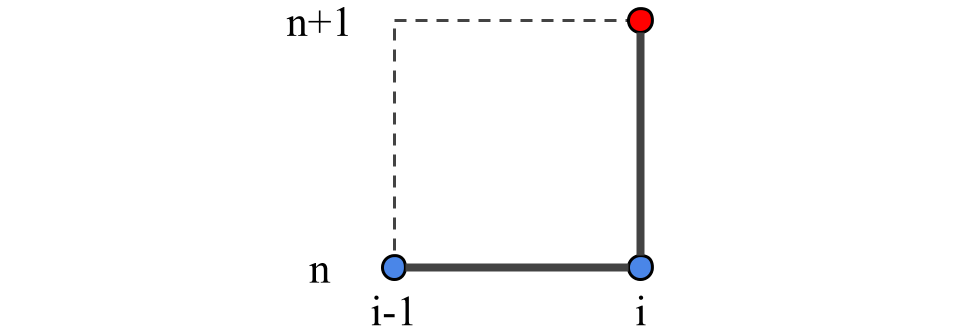
\includegraphics[height=3cm]{images/theory/scheme_cir.png}
    \caption{Шаблон схемы Куранта-Изаксона-Риса.}
    \label{fig:scheme_cir}
\end{figure}

\subsubsection{Схема Русанова}

Схема Русанова \cite{kholodov} для решения одномерного уравнения переноса \eqref{eq:lin_advection} имеет следующий вид:

\begin{equation}
    u_{i+1}^n = u_i^n + C\frac{\Delta_0 + \Delta_2}{2} + C^2 \dfrac{\Delta_0 - \Delta_2}{2} + C\left(C^2 - 1\right) \dfrac{\Delta_1 - 2\Delta_0 + \Delta+2}{6},
    \label{eq:rusanov}
\end{equation}

\noindent где

\begin{align*}
    & \Delta_0 = u_{i-1}^n - u_i^n, \\
    & \Delta_1 = u_{i-2}^n - u_{i-1}^n, \\
    & \Delta_2 = u_{i}^n - u_{i+1}^n .
\end{align*}

\noindent Схема Русанова имеет третий порядок аппроксимации и является монотонной по Годунову. Условие устойчивости схемы Русанова совпадает с условием уcтойчивости для схемы Куранта-Изаксона-Риса \eqref{eq:cfl_condition}.

Монотонность по Годунову означает, что данная схема переводит монотонный в момент времени $t_n$ профиль $u_i^n$ в монотонный в следующий момент времени $t_{n+1}$ профиль $u_i^{n+1}$. Это свойство позволяет применять схему Русанова для решения уравнения переноса даже при возникновении разрывных решений \cite{kholodov}.

\begin{figure}[!htb]
    \centering
    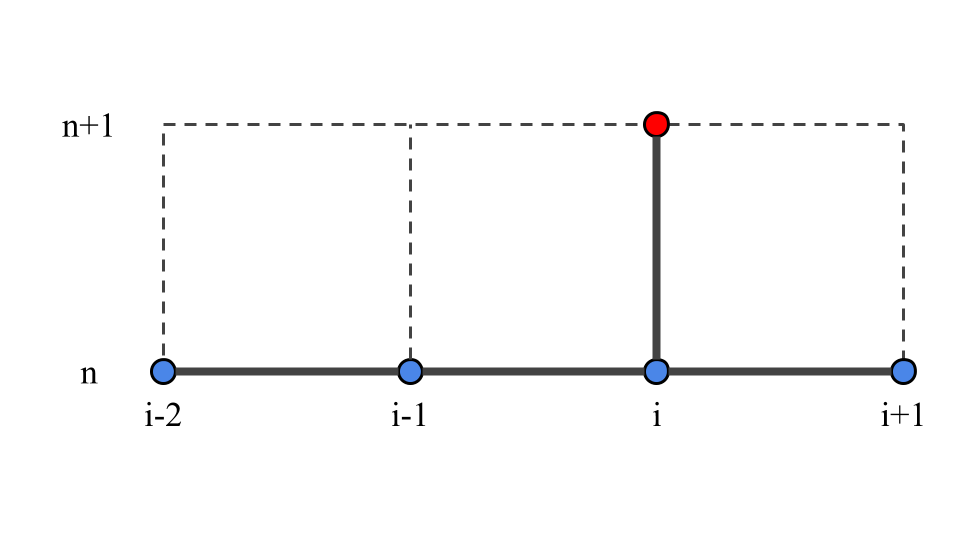
\includegraphics[height=3cm]{images/theory/scheme_rusanov.png}
    \caption{Шаблон схемы Русанова третьего порядка аппроксимации.}
    \label{fig:scheme_rusanov}
\end{figure}

\subsubsection{Схема TVD 2-го порядка аппроксимации}

Альтернативой монотонным по Годунову схемам являются TVD-схемы. Они также позволяют решать задачи с разрывами и большими градиентами, избегая появления осцилляций, вызванных дискретизацией задачи \cite{harten, rus_tvd, petrov_lobanov_book, kholodov}. 
Полная вариация (total variation) решения линейного уравнения переноса \eqref{eq:lin_advection} определяется как

\begin{equation*}
    \TV \left(q(\cdot, t)\right) = \int \left|\dfrac{\partial q}{\partial x}\right| dx .
\end{equation*}

\noindent Соответственно полная вариация численного решения задаётся как

\begin{equation*}
    \TV \left(q^n\right) = \TV \left(q(\cdot, t^n)\right) = \sum_i \left| q_{i+1}^n - q_i^n \right| .
\end{equation*}

\noindent Схема называется схемой с уменьшением полной вариации, или TVD-схемой (total varia\-tion diminishing scheme), или схемой, монотонной по Хартену, если

\begin{equation*}
    \TV \left(q^{n+1}\right) \leq \TV \left(q^n\right) .
\end{equation*}

В некоторых расчётах мы будем использовать TVD-схему 2-го порядка:

\begin{equation}
\begin{dcases}
    q_i^{n+1} = q_i^n - \dfrac{\tau}{h}\left(f_{i+\sfrac{1}{2}} - f_{i-\sfrac{1}{2}}\right) , \\
    f_{i+\sfrac{1}{2}} = \dfrac{f_i^n + f^n_{i+1}}{2} - \dfrac{\theta}{2}\left(f_{i+1}^n - f_i^n\right) + \dfrac{\phi_{sb}(r_i)}{2} \left(\theta - C\right) \left(f_{i+1}^n - f_i^n\right) , \\
    \theta = \sign C_{i+\sfrac{1}{2}} ,
\end{dcases}
\label{eq:tvd_scheme}
\end{equation}
 
\noindent где $\phi_{sb}(r_i)$ --- ограничитель потока  superbee
\begin{equation*}
    \phi_{sb}(r_i) = \max \left\{0, \min\{2r_i,1\}, \min\{r_i,2\}\right\} , 
\end{equation*}
\begin{equation*}
    r_i = \dfrac{q_i - q_{i-1}}{q_{i+1} - q_i} .
\end{equation*}

\subsection{Моделирование воздействия бура}

\subsubsection{Постановка численного эксперимента}

Будем рассматривать геологическую модель с газовым слоем (\autoref{fig:island}). Для представления каждого слоя будем использовать регулярные прямоугольные сетки с протранственным шагом 0.5\texttimes 0.5 м Для расчётов применим схему Русанова третьего порядка \eqref{eq:rusanov} с шагом по времени 0.05 мс. Выполним 14 тыс. шагов по времени, чтобы пронаблюдать отражение волны, испущенной точечным источником, от газоносного слоя и далее от свободной поверхности льда.

\subsubsection{Результаты}

Распространение волны от бура можно условно разделить на три  отрезка. Первый --- начальное движение почти  сферической волны от источника с активным проникновением в ледовый остров (\autoref{fig:wave_image}). Второй --- движение волны вглубь твёрдой породы и обратное движение после отражения от газоносного слоя (\autoref{fig:wave_image_2}). Третий --- движение волны вверх по придонному слою с последующим проникновением в остров и отражением от свободной поверхности льда (\autoref{fig:wave_image_3}).

Можно заметить (см. \autoref{fig:wave_image}), что ледовый остров играет роль своеобразного резонатора. Свободная поверхность льда является полностью отражающей, в то время как граница между льдом и придонным слоем отражает упругие волны частично. Так как высота острова мала по сравнению с его длиной, то за время, которое требуется  горизонтально распространяющейся волне для достижения края острова, вертикально распространяющаяся волна испытывает множество переотражений. Это означает, что, возможно, при некотором специальном выборе внешнего периодического возмущения, ледовый остров способен накапливать упругие волны. Накопление, естественно, будет происходить до момента начала разрушения льда. Такое резонансное явление, если оно существует, представляет существенную опасность для работ на подобной ледовой платформе.

Если волна, распространяющаяся от введённого точечного источника, имеет большую амплитуду, то она способна разрушить лёд. Как видно из \autoref{fig:wave_image}, такие разрушения будут вероятно локализованы непосредственно над точкой бурения. Этому способствует интерференция волн, входящих в остров снизу, с волнами, отражающимися от свободной поверхности льда. Волновая картина на \autoref{fig:wave_image_3} свидетельствует о том, что разрушения возникнут сразу после начала бурения --- волна, отражённая от газоносного слоя, имеет гораздо меньшую амплитуду по сравнению с первоначальной волной.

\begin{figure}[!h]
    \centering
    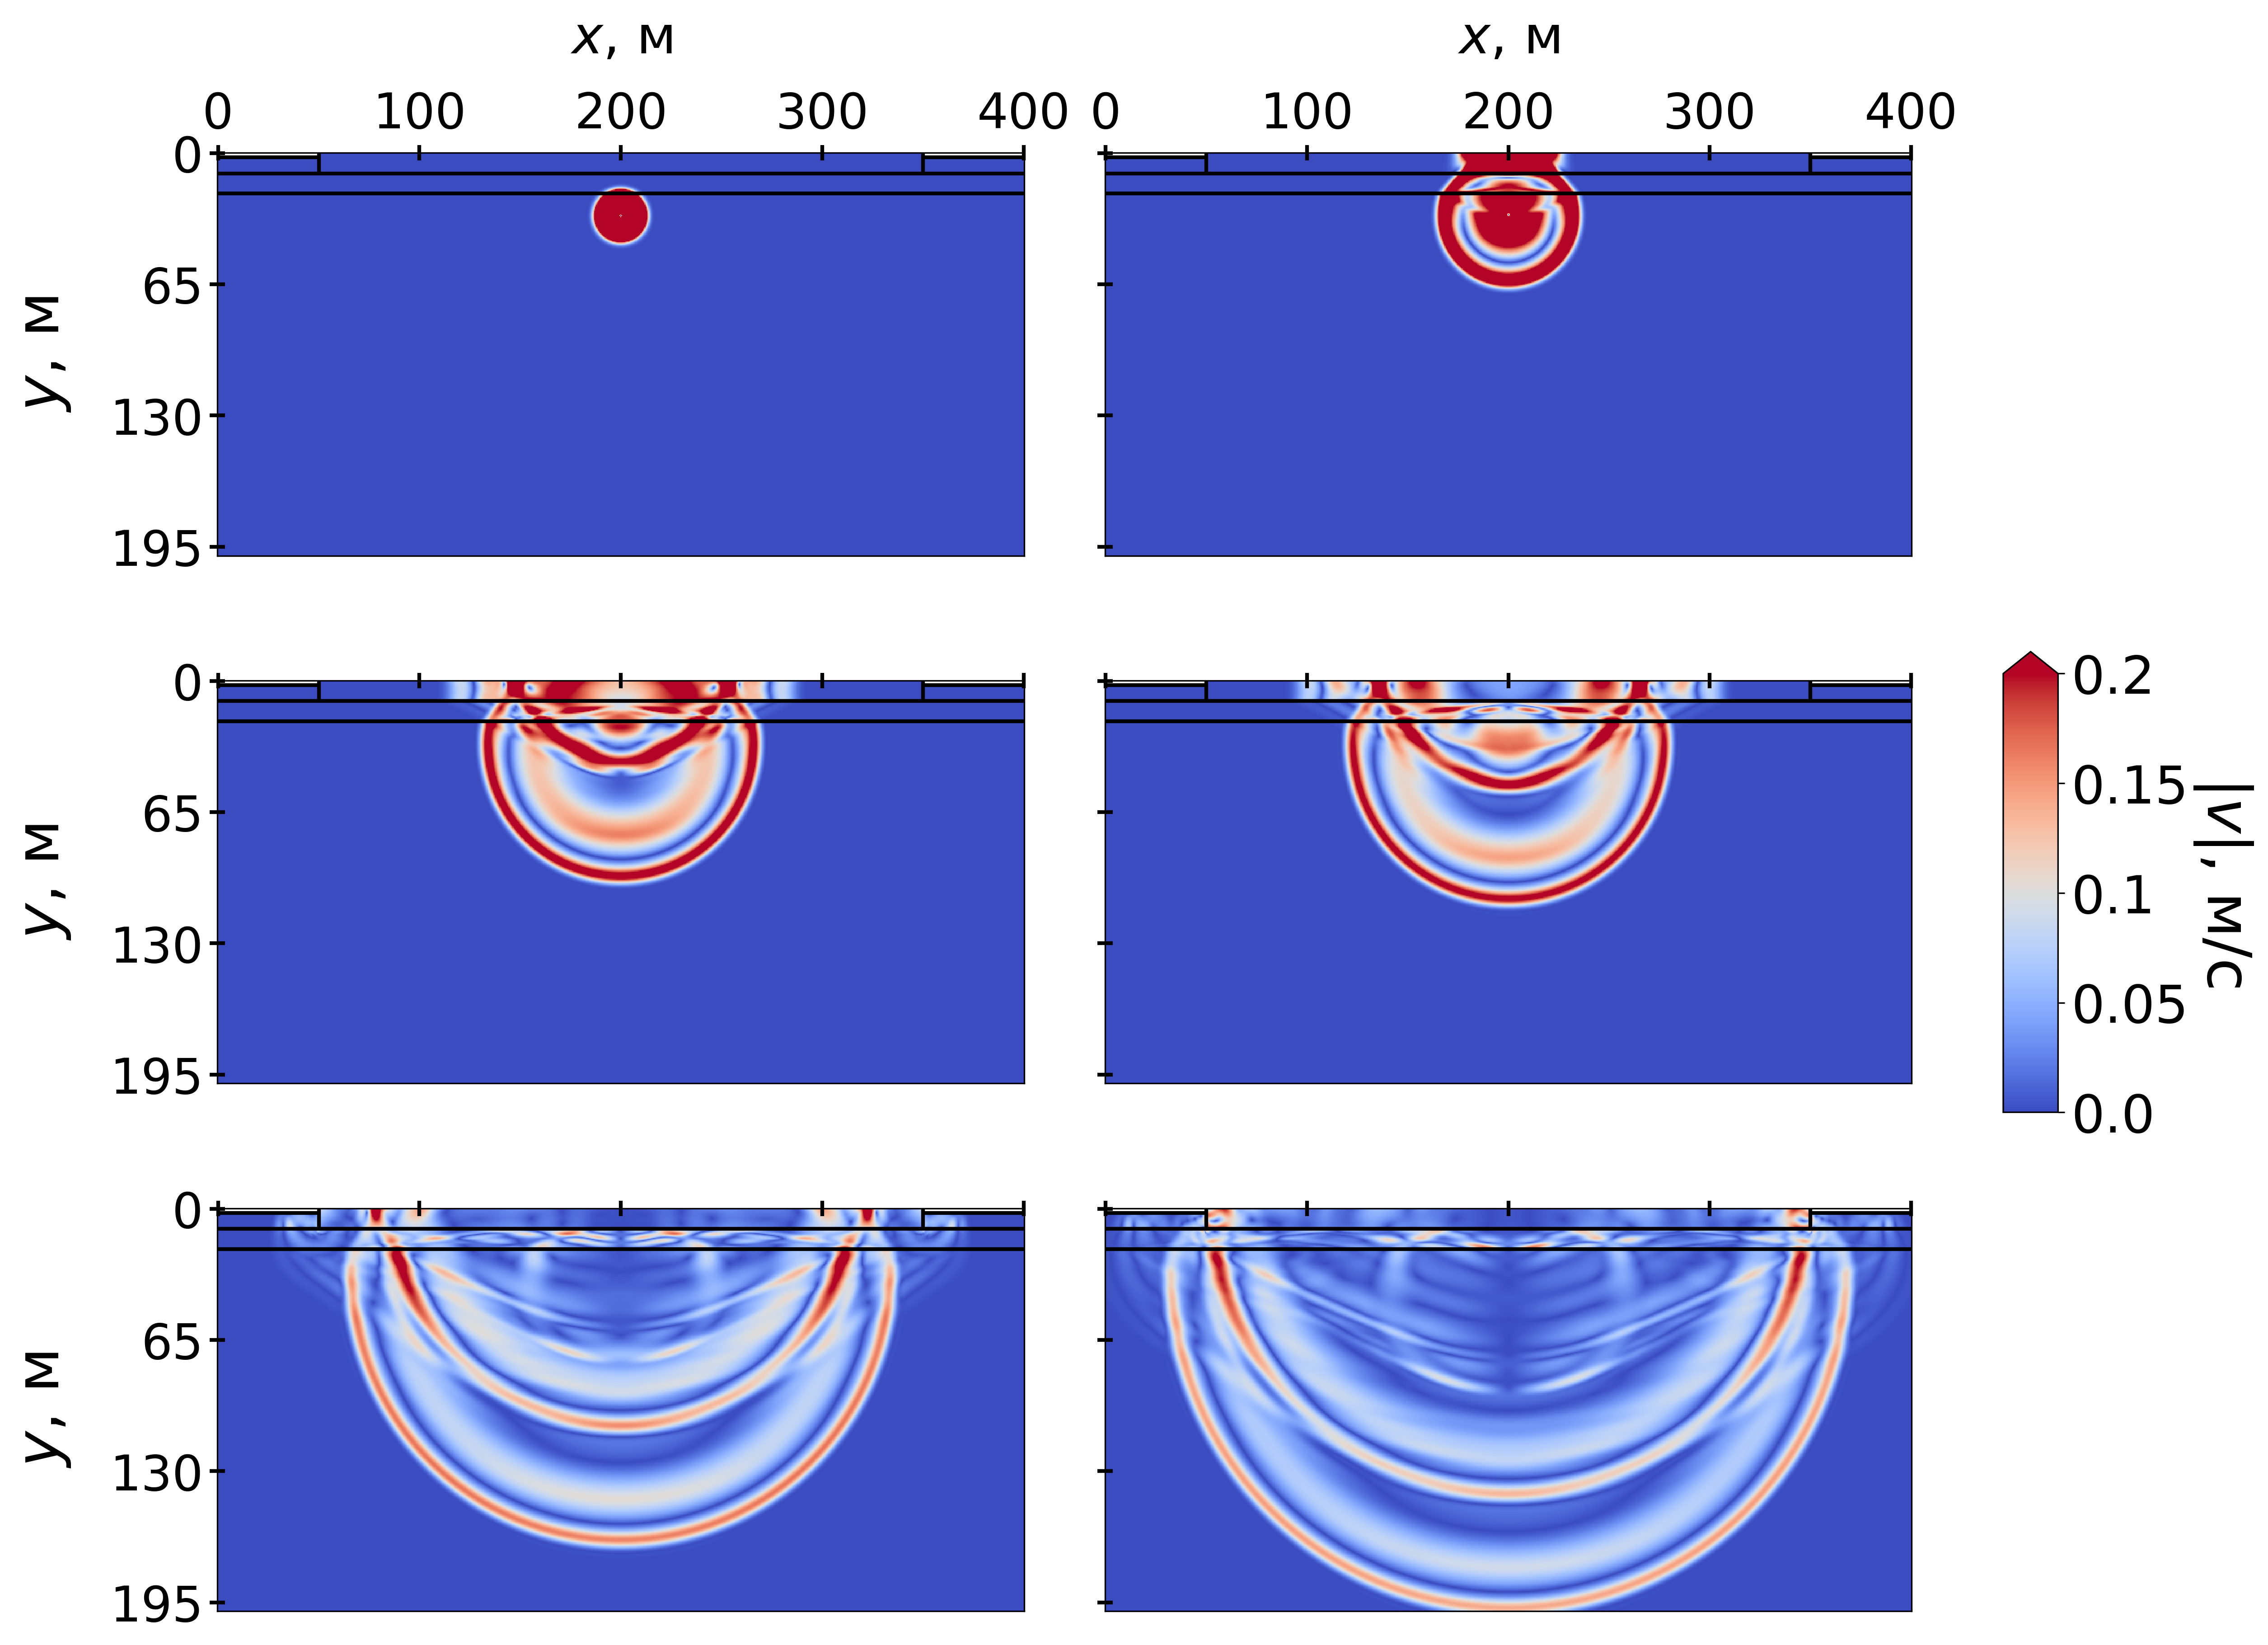
\includegraphics[width=\textwidth]{images/gas_field/wave_pic_1.png}
    \caption{Волновая картина в моменты времени 0.005, 0.020, 0.035, 0.050 и 0.075 сек. (слева--направо и сверху--вниз).}
    \label{fig:wave_image}
\end{figure}

Можно заметить (см. \autoref{fig:wave_image_2}), что структура волны, отражённой от газового слоя, является довольно регулярной. Это может быть в дальнейшем использовано, например, для решения обратной задачи сейсморазведки или для определения дефектов льда.

\begin{figure}[H]
    \centering
    \begin{subfigure}{0.49\textwidth}
        \centering
        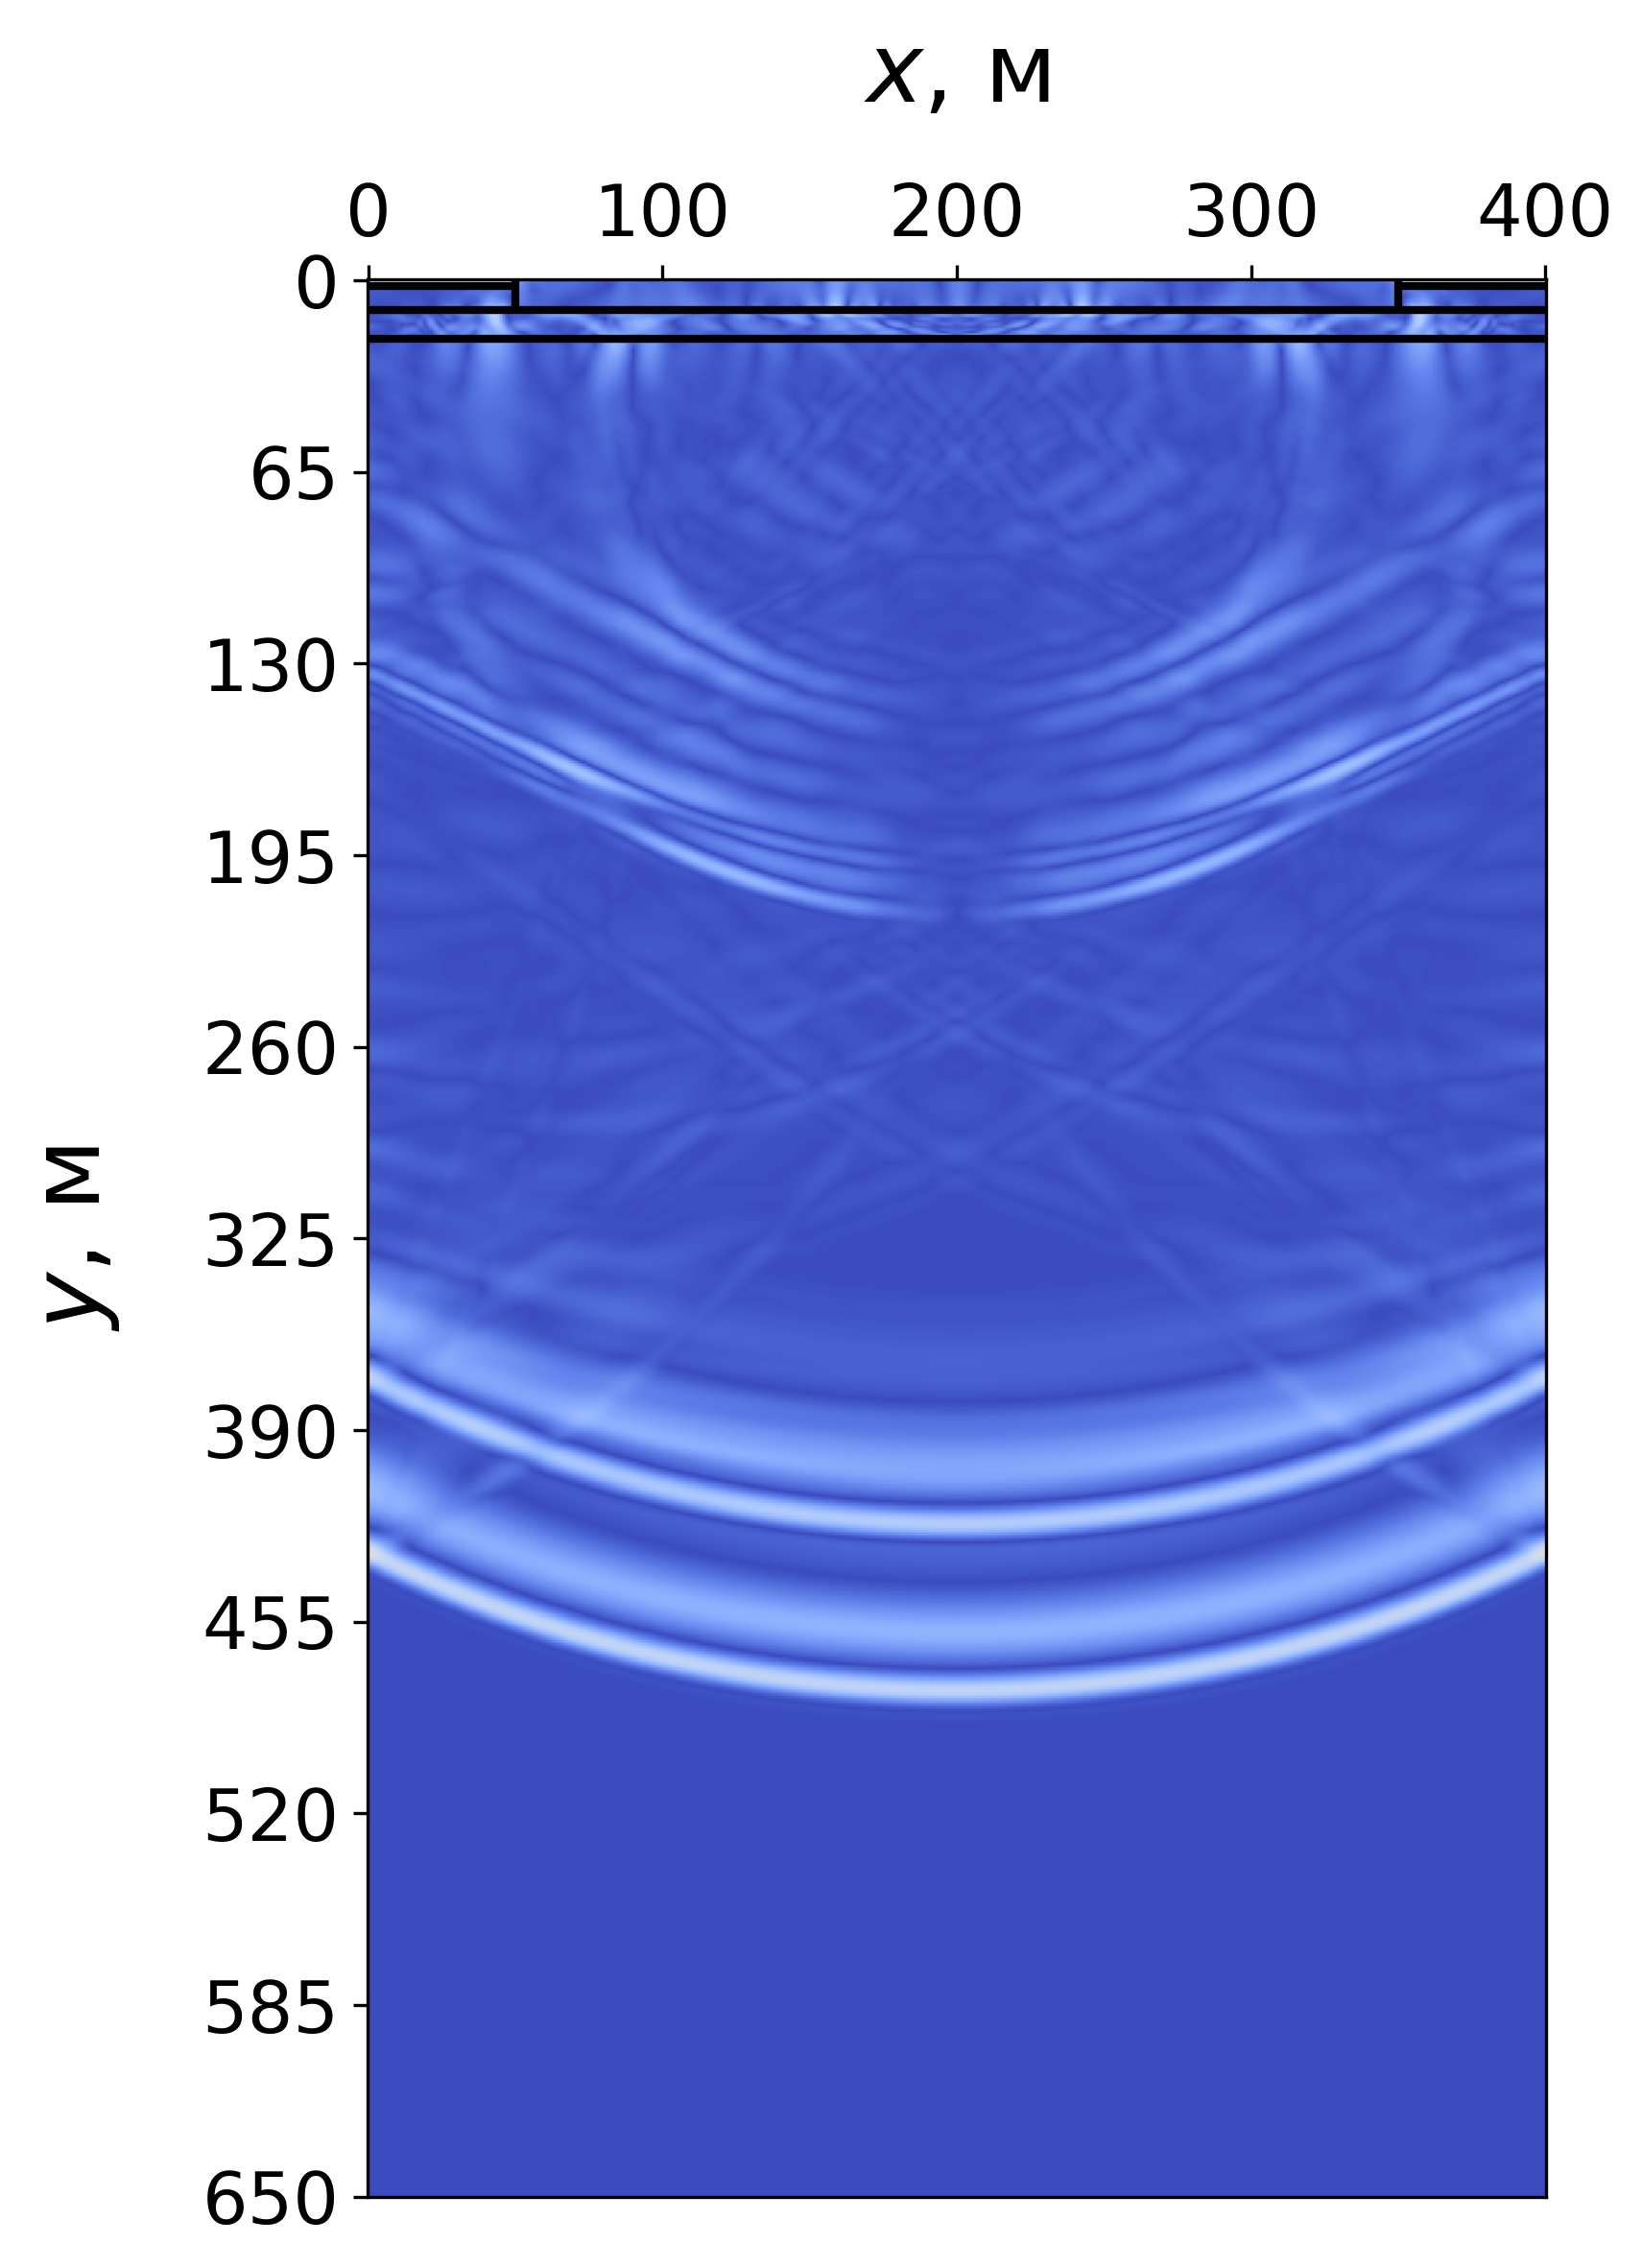
\includegraphics[width=\textwidth]{images/gas_field/004000.png}
    \end{subfigure}
    \hfill
    \begin{subfigure}{0.49\textwidth}
        \centering
        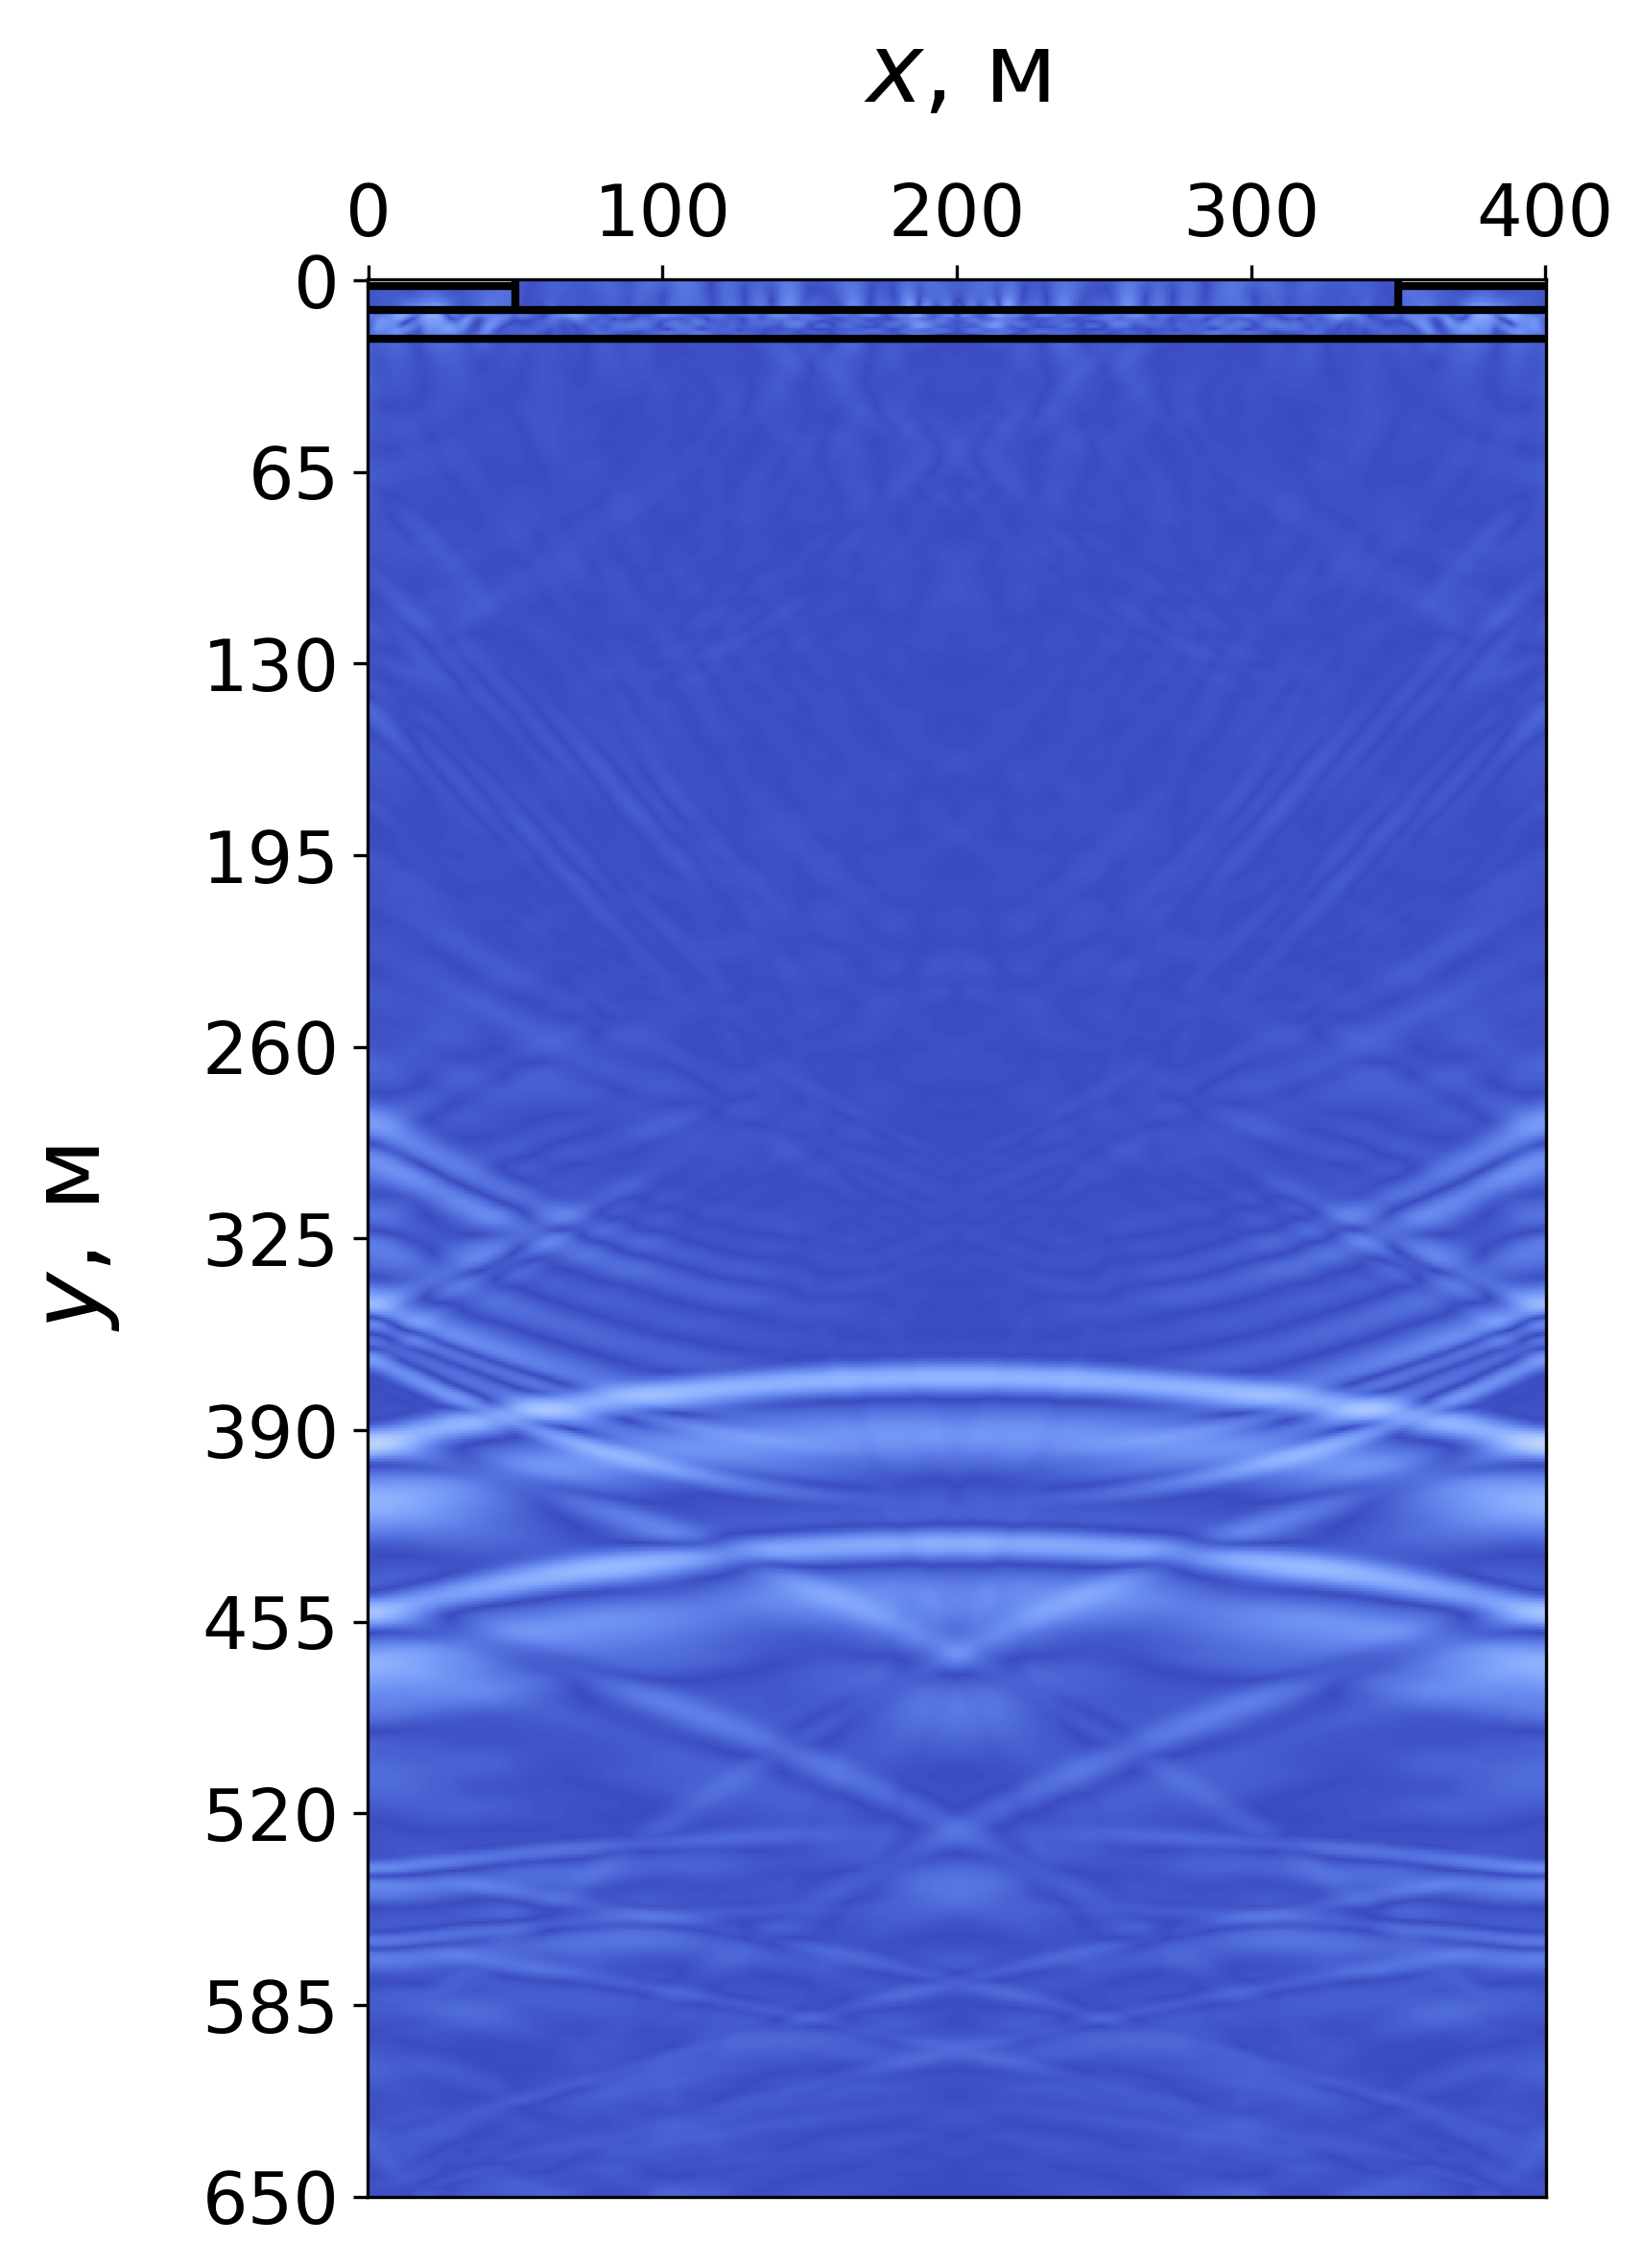
\includegraphics[width=\textwidth]{images/gas_field/008000.png}
    \end{subfigure}
    \caption[Волновая картина в моменты времени 0.2 и 0.35 сек. (слева--направо).]{Волновая картина в моменты времени 0.2 и 0.35 сек. (слева--направо)\protect\footnotemark.}
    \label{fig:wave_image_2}
\end{figure}

\footnotetext{\label{fn:cmap}Здесь используется та же цветовая гамма, что и в \autoref{fig:wave_image}.}

\begin{figure}[H]
    \centering
    \begin{subfigure}{0.49\textwidth}
        \centering
        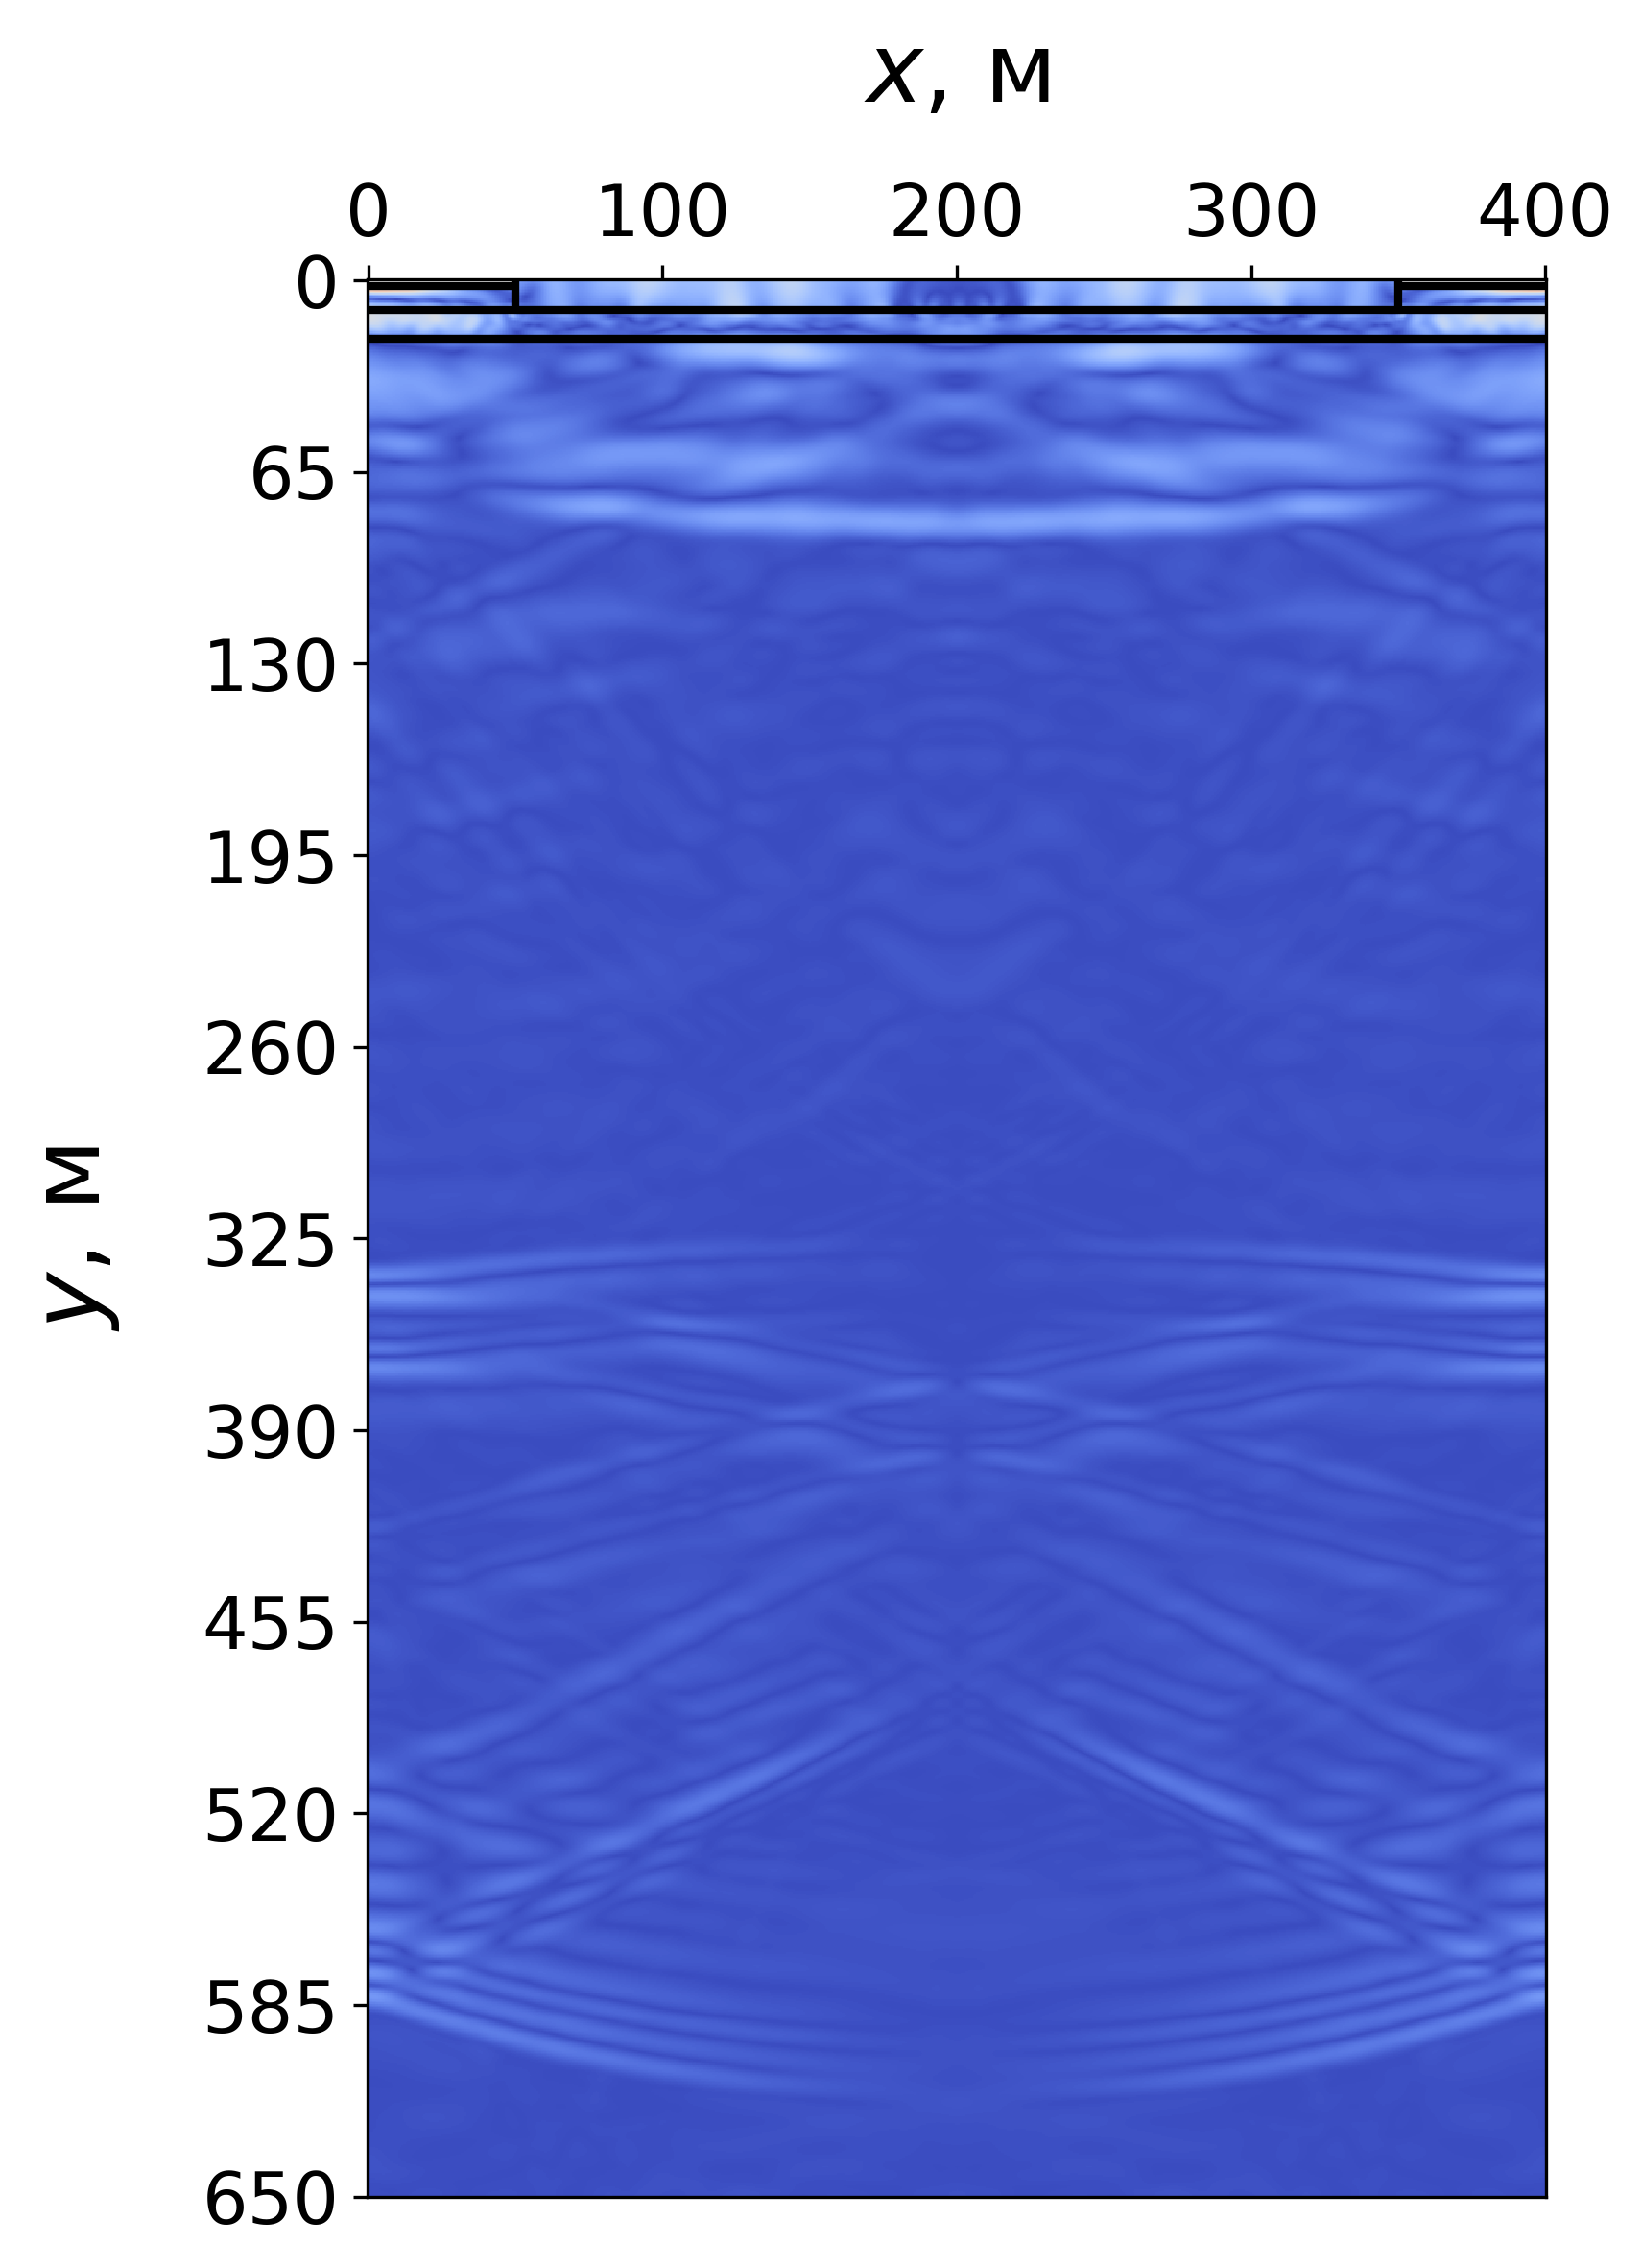
\includegraphics[width=\textwidth]{images/gas_field/012000.png}
    \end{subfigure}
    \hfill
    \begin{subfigure}{0.49\textwidth}
        \centering
        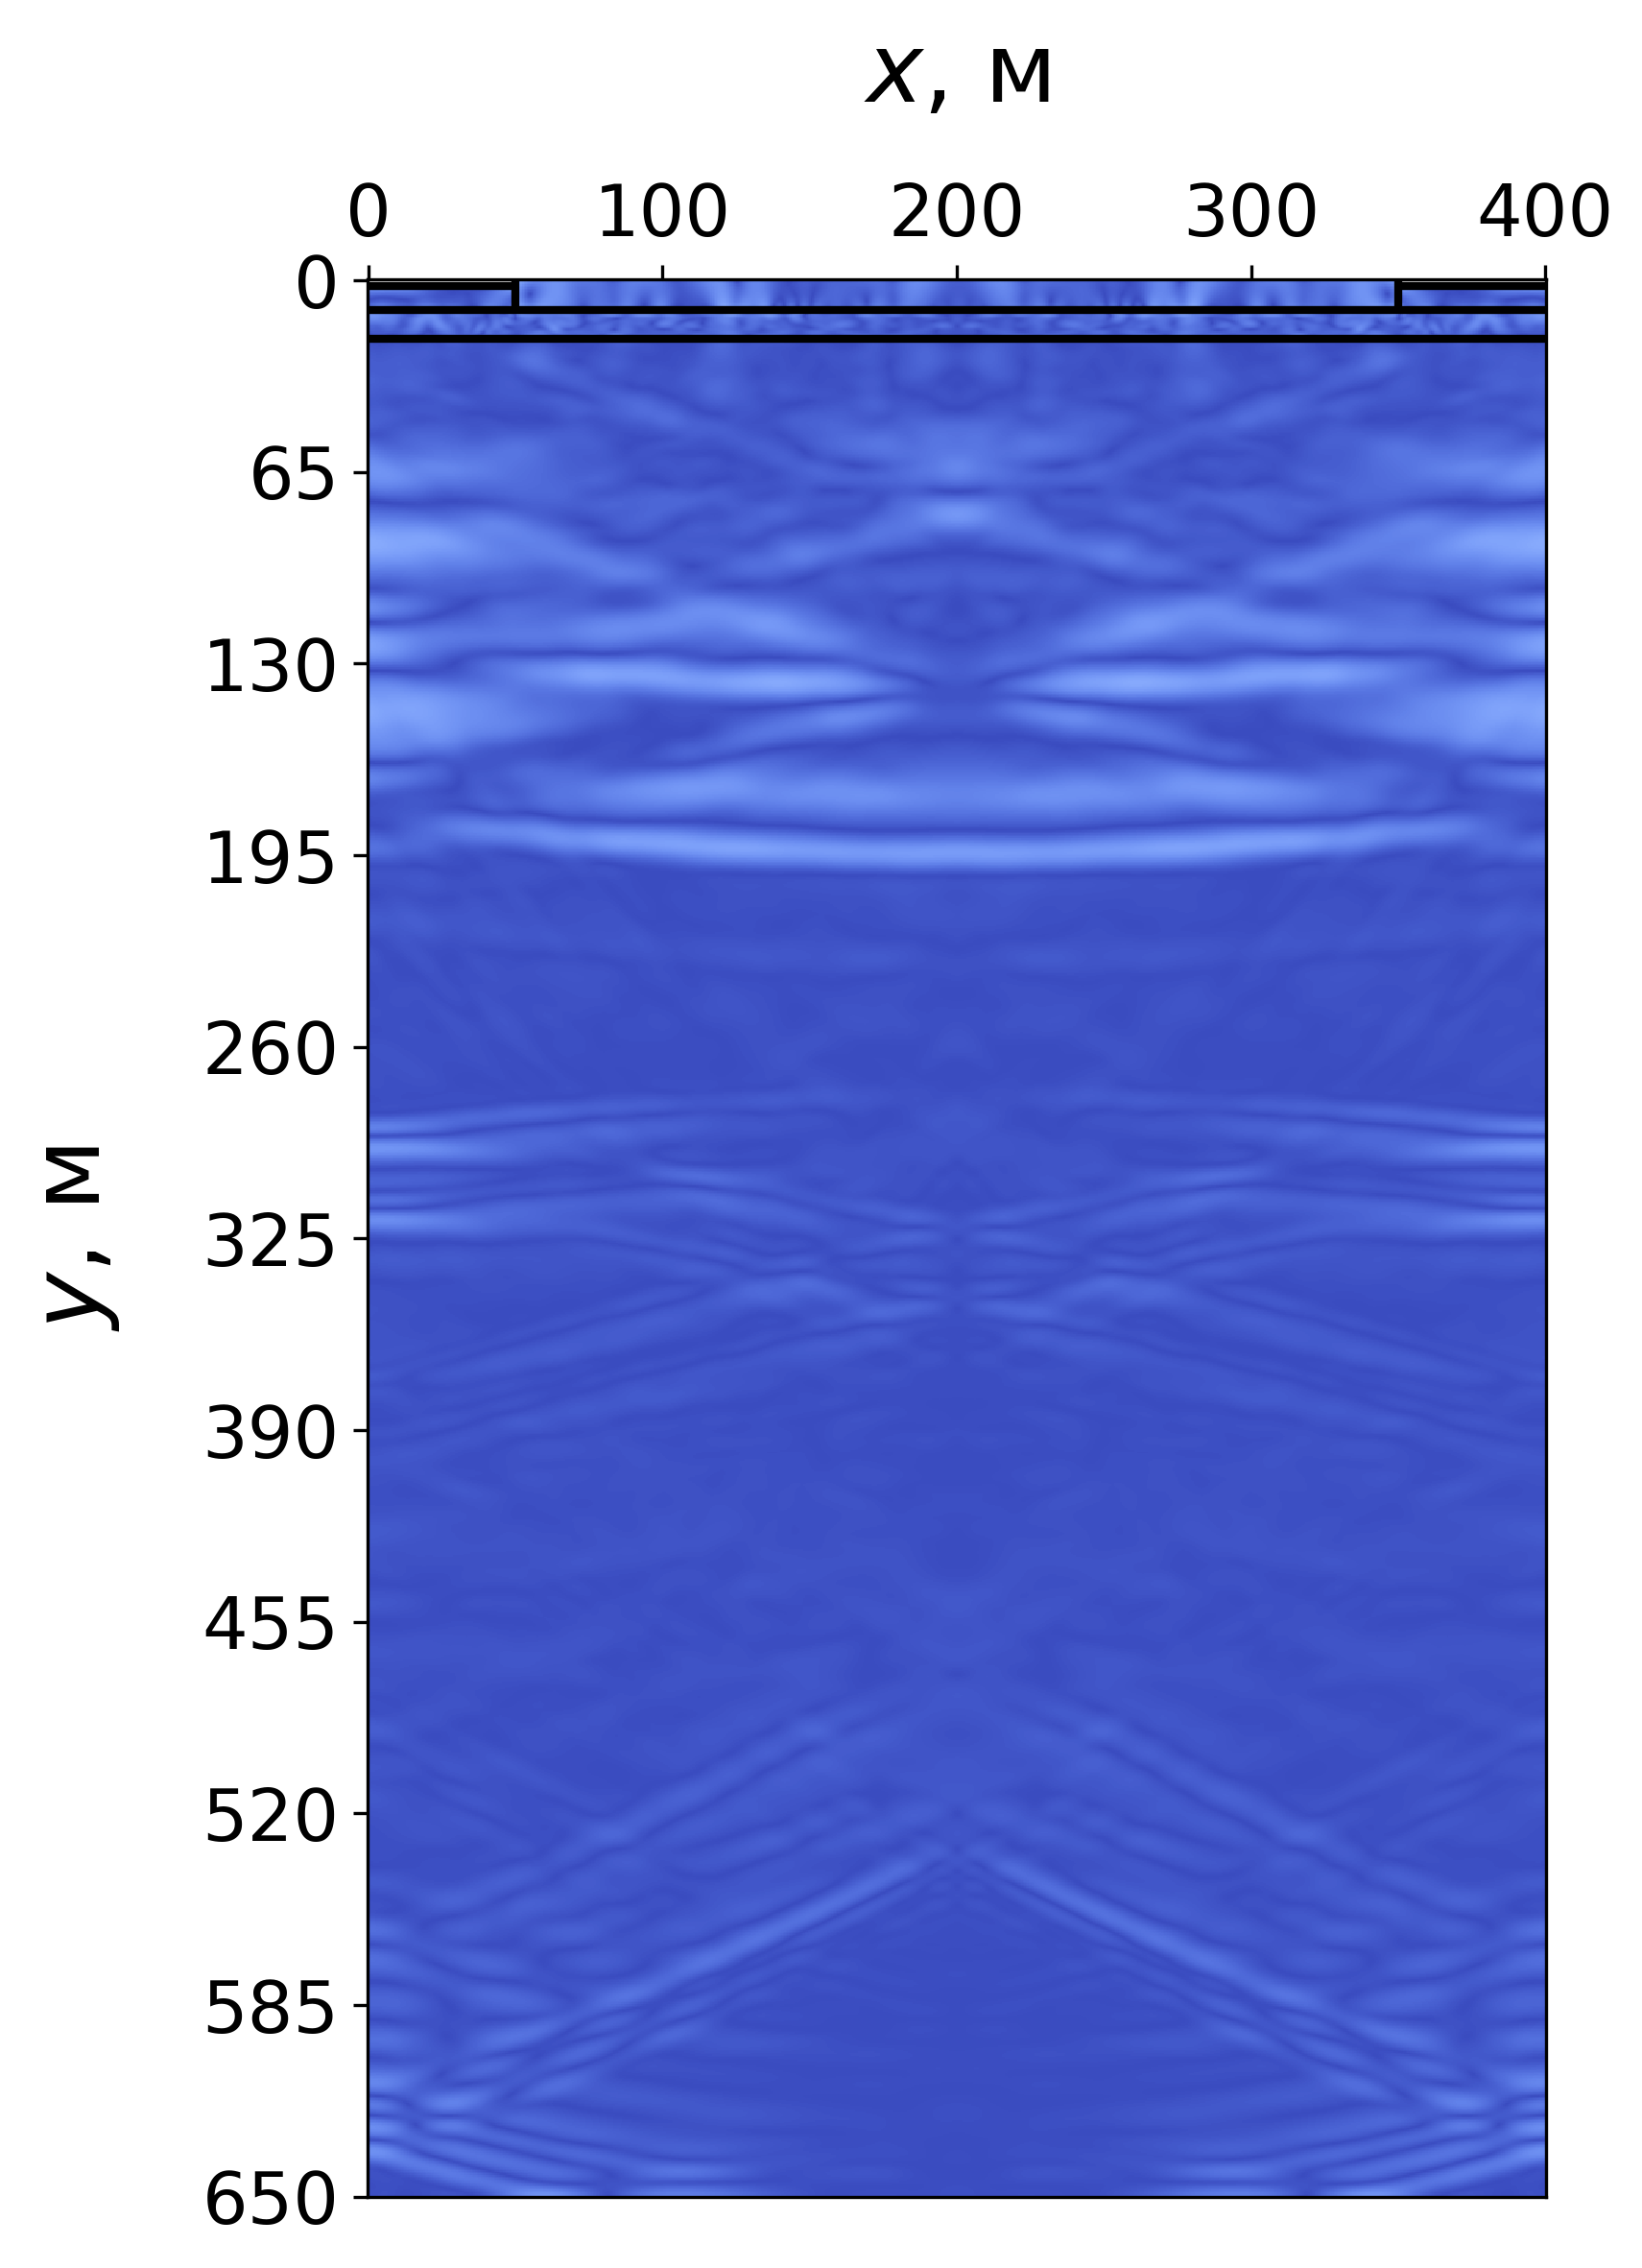
\includegraphics[width=\textwidth]{images/gas_field/013000.png}
    \end{subfigure}
    \caption{Волновая картина в моменты времени 0.6 и 0.65 сек. (слева--направо)\textsuperscript{\ref{fn:cmap}}.}
    \label{fig:wave_image_3}
\end{figure}

\subsection{Моделирование статической нагрузки}

\subsubsection{Постановка численного эксперимента}

Для решения задачи о распределении статической нагрузки (см. \autoref{fig:stamp_scheme}), воспользуемся методом установления \cite{fedorenko_relaxation}, решая при этом те же системы дифференциальных уравнений в частных производных \eqref{eq:acoustic_wave_eq} и \eqref{eq:elastic_wave_eq}. Будем считать распределение напряжений в ледовом острове установившимся, если модуль скорости распространения упругих волн оказывается в конечный момент времени в 20--30 раз меньше по сравнению со значением скорости в начальный момент.

Будем считать, что здание\footnote{Здесь под <<зданием>> мы понимаем некоторую покоящуюся конструкцию. Это может быть, например, техническое помещение, буровая установка или тяжёлое транспортное средство.}, расположенное на поверхности ледового острова, имеет массу 100 тонн и основание 5\texttimes 5 метров, тем самым производя на лёд давление величиной 4 кПа.

Будем использовать схему Куранта-Изак\-сона-Риса первого порядка \eqref{eq:cir_scheme} на регулярных прямоугольных сетках с пространственным шагом 0.5\texttimes 0.5 м и шагом по времени 0.02 мс. 

\subsubsection{Результаты}

После выполнения 200 тысяч шагов модуль скорости уменьшился примерно в 33 раза с $2.4\cdot10^{-4}$ м/c до $7.3\cdot10^{-6}$ м/c. Таким образом, получившиеся распределения напряжений можно считать установившимся.

Так как внешними условиями задано только давление здания на горизонтальную поверхность льда, то естественно, что $\sigma_{yy}$ будет составлять большую часть от итогового суммарного давления $p$ и, соответственно, напряжения фон Мизеса $\sigma_\nu$. Для того, чтобы в этом убедиться, достаточно сравнить распределение $\sigma_{yy}$, изображённое на \autoref{fig:stamp_syy}, с распределениями горизонтальной и смешанной компонент тензора напряжений $\sigma_{xx}$ и $\sigma_{xy}$, представленными на \autoref{fig:stamp_sxx} и \autoref{fig:stamp_sxy}.

Из распределения давлений $p$ (\autoref{fig:stamp_p}) и напряжения фон Мизеса (\autoref{fig:stamp_mises}) хорошо видно, что, кроме цилиндрической области непосредственно под зданием, наиболее подверженными разрушению областями являются конусообразные области радиусом около 20 метров, находящиеся в приблизительно 2 метрах от поверхности. Вблизи свободной поверхности данные области подвержены растягивающим напряжениям (см. \autoref{fig:stamp_p}), а вблизи границы с придонным слоем --- сдавливающим.

Максимальное достигаемое напряжение фон Мизеса 

\begin{equation*}
    \max_{i,j} \sigma_\nu\left(x_i, y_j\right) \approx 2.2~ \text{кПа} .
\end{equation*}

\noindent много меньше предела сдвигового напряжения льда, равного $y_s = 1~\text{Мпа}$. Таким образом, при реалистичных значениях статической нагрузки лёд разрушаться не будет.

\begin{figure}[H]
    \centering
    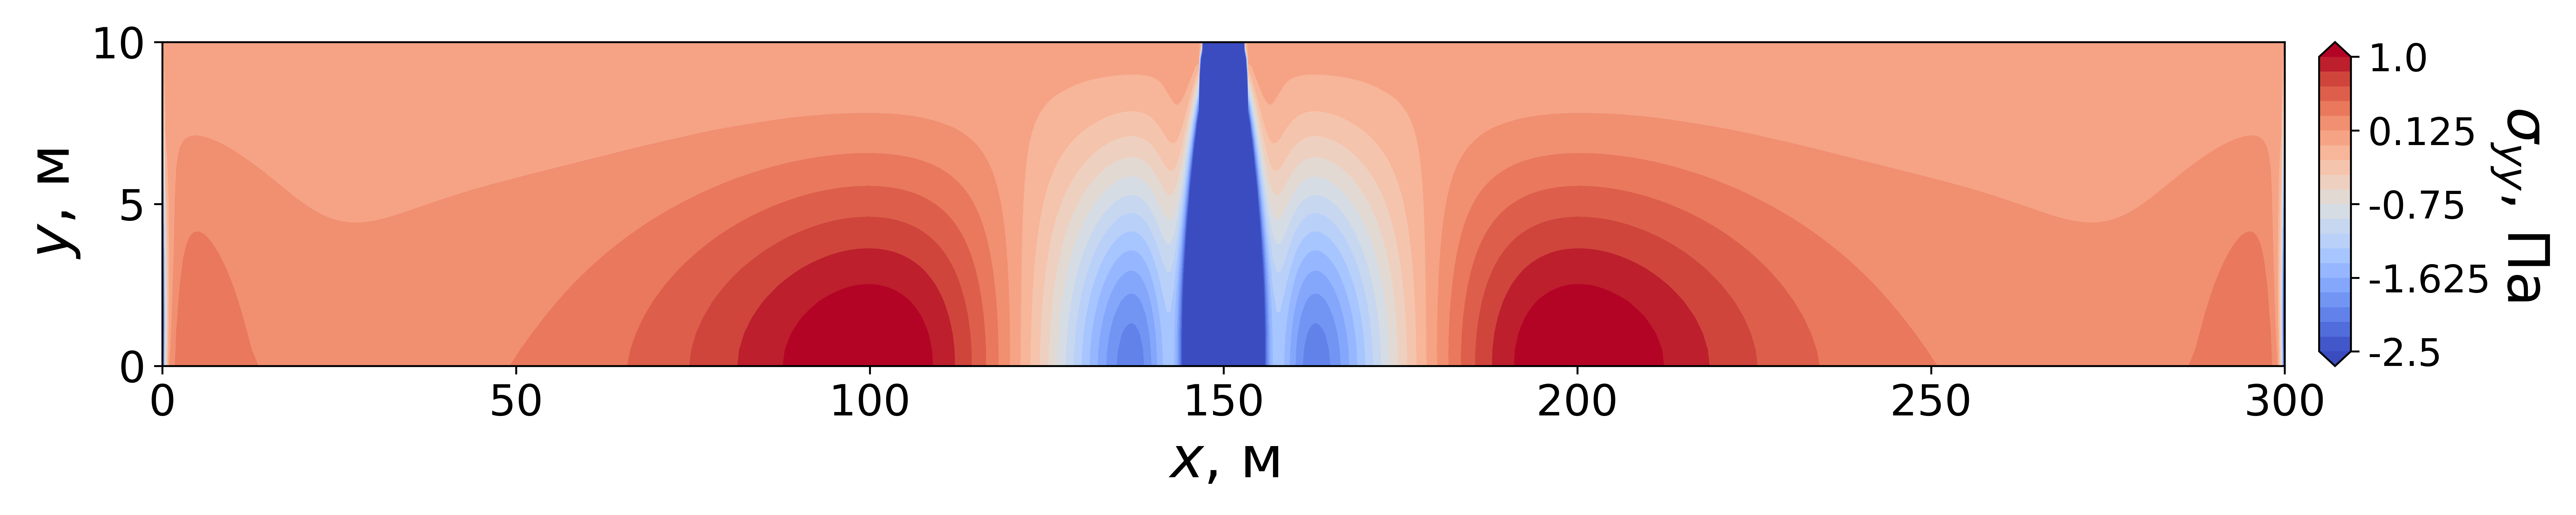
\includegraphics[width=\textwidth]{images/stamp/stamp_syy.png}
    \caption{Распределение вертикальной компоненты тензора напряжений $\sigma_{yy}$.}
    \label{fig:stamp_syy}
\end{figure}

\begin{figure}[H]
    \centering
    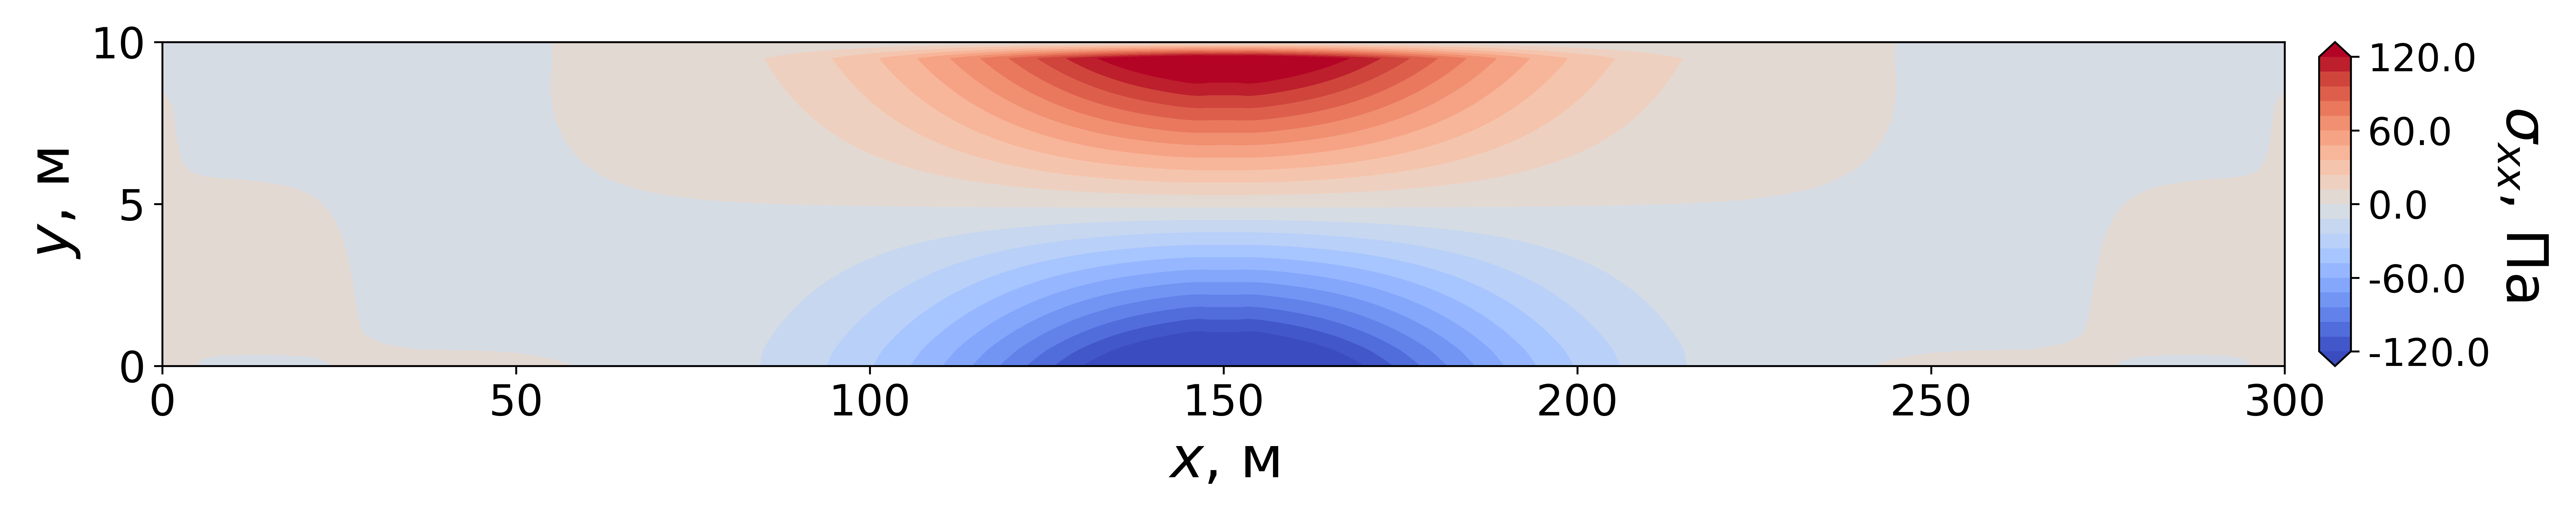
\includegraphics[width=\textwidth]{images/stamp/stamp_sxx.png}
    \caption{Распределение горизонтальной компоненты тензора напряжений $\sigma_{xx}$.}
    \label{fig:stamp_sxx}
\end{figure}

\begin{figure}[H]
    \centering
    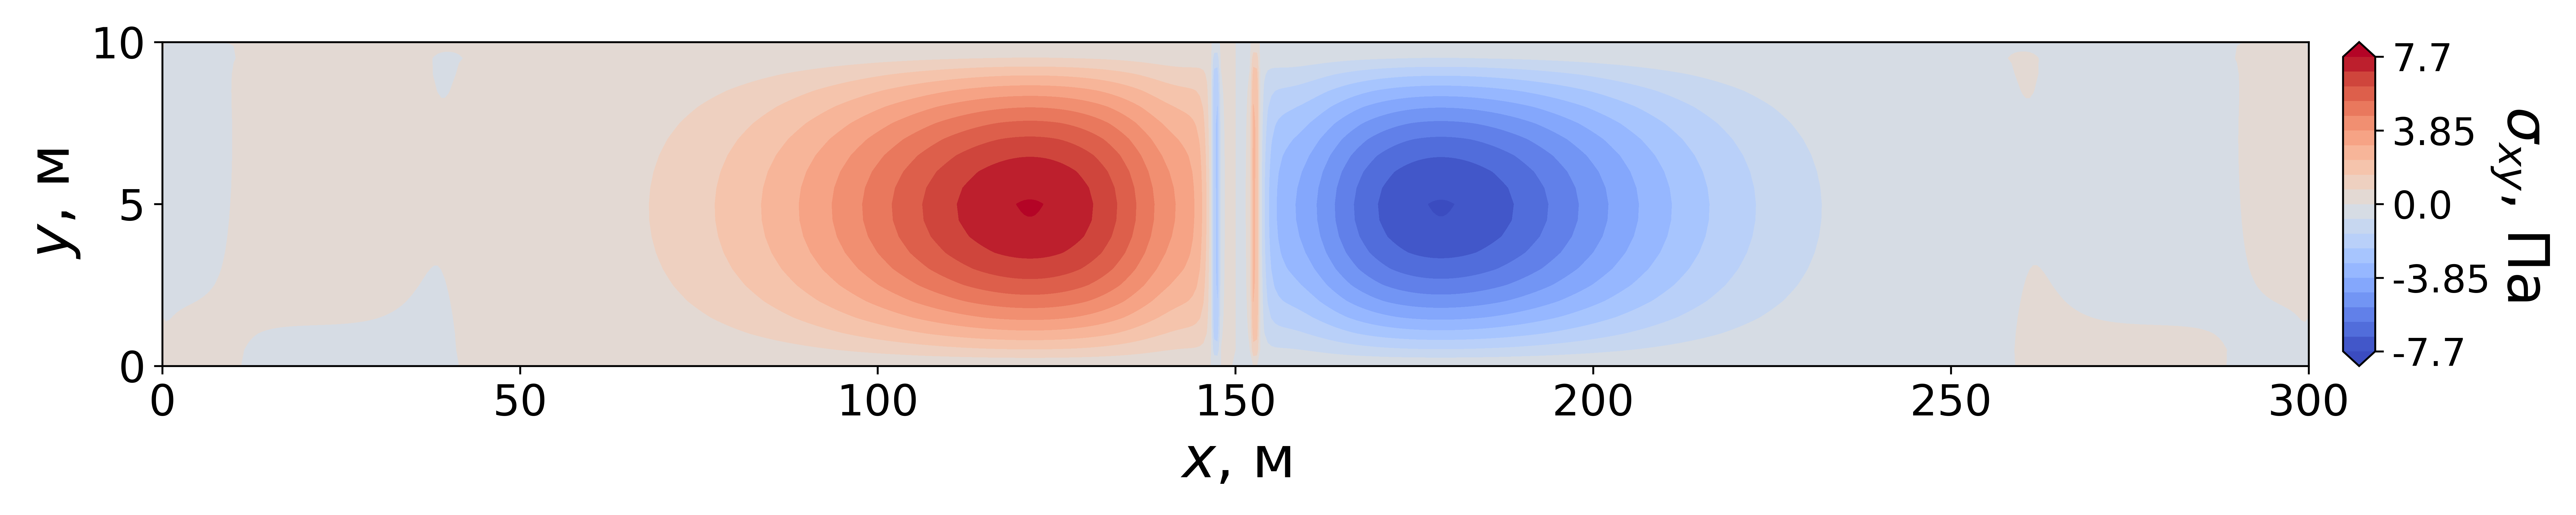
\includegraphics[width=\textwidth]{images/stamp/stamp_sxy.png}
    \caption{Распределение смешанной компоненты тензора напряжений $\sigma_{xy}$.}
    \label{fig:stamp_sxy}
\end{figure}

\begin{figure}[H]
    \centering
    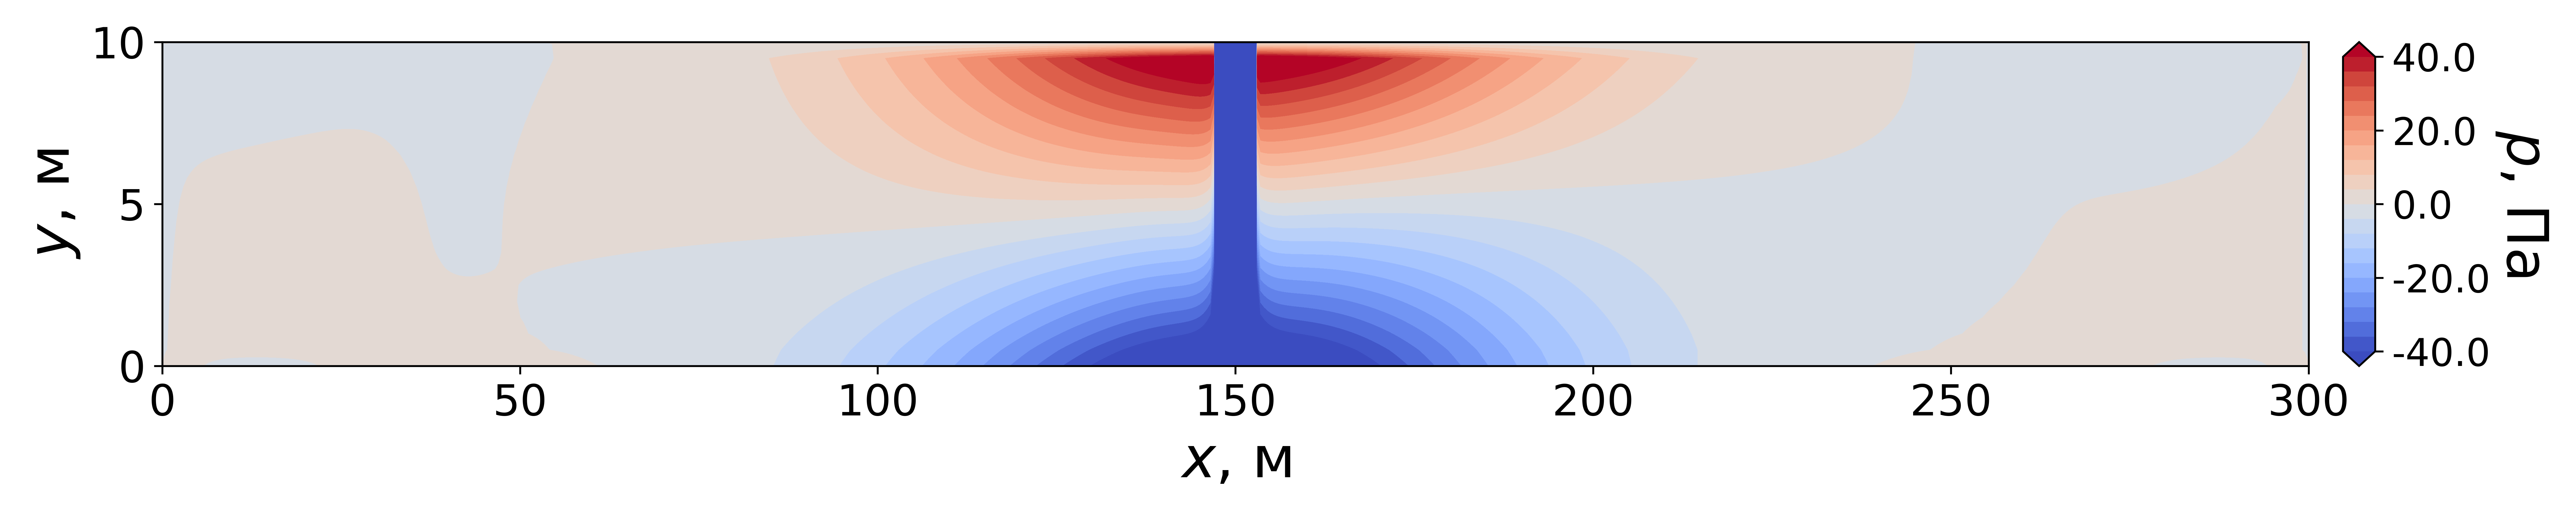
\includegraphics[width=\textwidth]{images/stamp/stamp_p.png}
    \caption{Распределение давления $p$.}
    \label{fig:stamp_p}
\end{figure}

\begin{figure}[H]
    \centering
    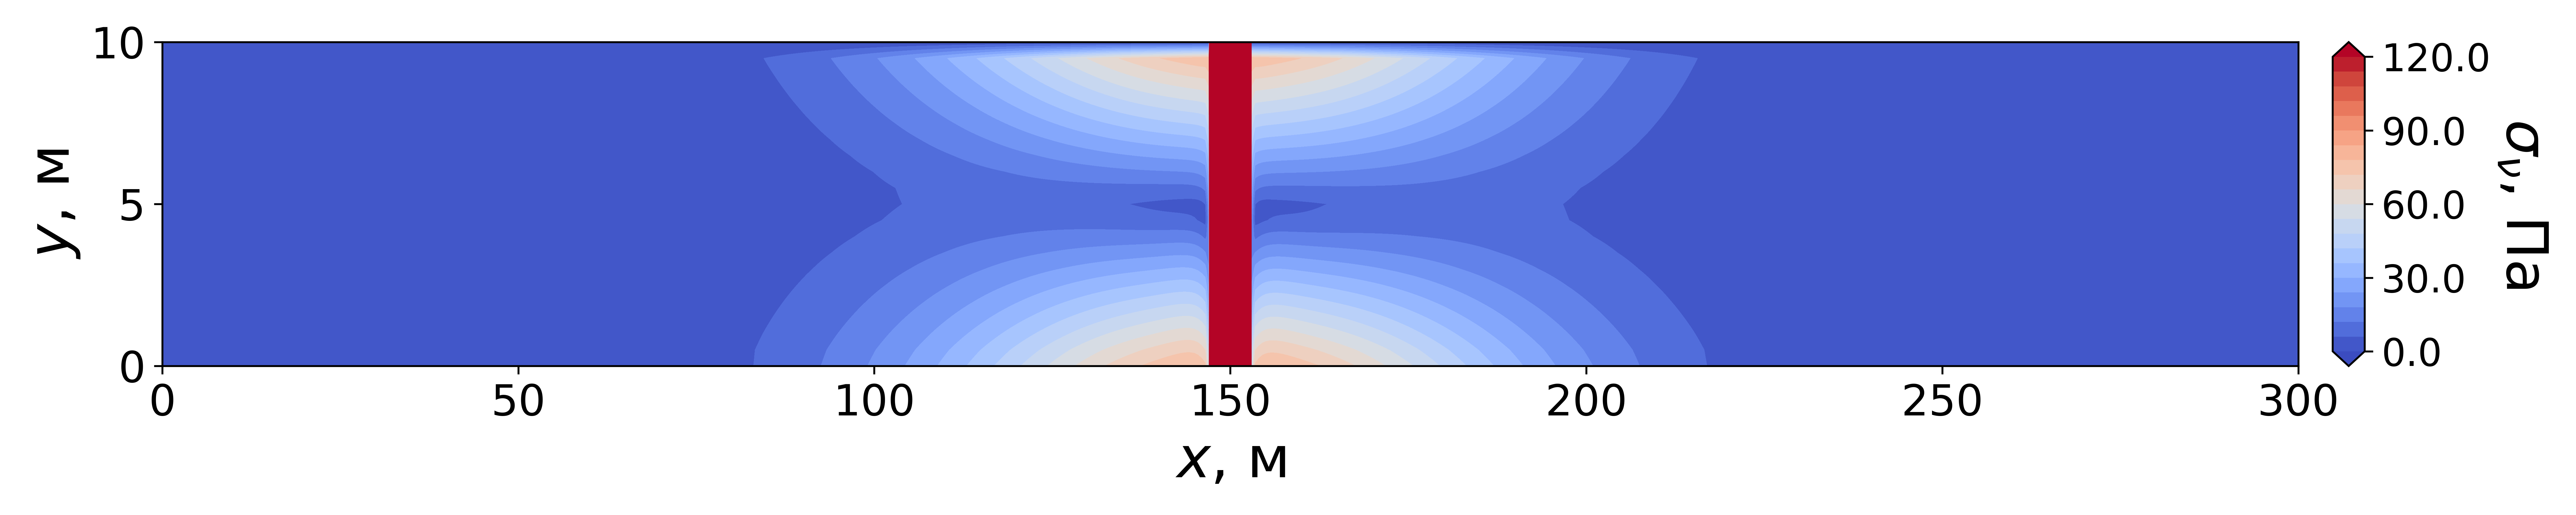
\includegraphics[width=\textwidth]{images/stamp/stamp_mises.png}
    \caption{Распределение напряжения фон Мизеса $\sigma_\nu$.}
    \label{fig:stamp_mises}
\end{figure}
